\def\HandoutMode{}
\def\NotesSecondScreen{1}
\def\ButtonsMode{1}
\def\ScriptMode{1}
\documentclass[\HandoutMode,table]{beamer}

\mode<presentation>
\usetheme{CambridgeUS}
\usecolortheme{seahorse}

\usepackage[english]{babel}
\usepackage[utf8]{inputenc}
\usepackage[T1]{fontenc}
\usepackage{xspace}
\usepackage[noend]{algorithm2e}
\usepackage{listings}
\usepackage{graphicx}
\usepackage{pgfpages,pgfopts}
\usepackage{ifthen}
\usepackage{xstring}
\usepackage{calc}

\usepackage{tikz}
\usepackage{smartdiagram}
\usepackage{tikz-uml}
\usetikzlibrary{positioning}
\usesmartdiagramlibrary{additions}
% dirty hack to make smartdiagram and tikz-uml work together
\pgfsetlayers{background,smart diagram arrow back,%
    component0,component1,component2,connections,main}

\usepackage{xcolor}
\usepackage{booktabs}
\usepackage{subfig}
\usepackage[justification=centering,format=hang]{caption}
\usepackage{adjustbox}
\usepackage{mathtools}
\usepackage{comment}

\ifthenelse{\equal{\HandoutMode}{handout}}{%
    \pgfpagesuselayout{2 on 1}[a4paper,border shrink=5mm]
}{%
    \ifthenelse{\not\equal{\NotesSecondScreen}{}}{%
        \setbeameroption{show notes on second screen=right}
    }{}
}

\ifthenelse{\equal{\ScriptMode}{}}
{%
    \newcommand<>{\script}[1]{}
    \providecommand\slideintonotemag{.5}
}
{%
    \newcommand<>{\script}[1]{\note#2{#1}}
    \providecommand\slideintonotemag{.3}
}

\newcommand{\myTitle}{Uberfuzz\xspace}
\newcommand{\mySubtitle}{A Cooperative Fuzzing Framework\xspace}
\newcommand{\myDegree}{Master of Science in Artificial Intelligence\xspace}
\newcommand{\myName}{Andrea Jemmett\xspace}
\newcommand{\myProf}{Dr. Sanjay Rawat\xspace}
\newcommand{\myOtherProf}{Put name here\xspace}
\newcommand{\mySupervisor}{Put name here\xspace}
\newcommand{\myFaculty}{Faculty of Science\xspace}
\newcommand{\myDepartment}{Dept.\ of Computer Science\xspace}
\newcommand{\myUni}{Vrije Universiteit Amsterdam\xspace}
\newcommand{\myLocation}{Amsterdam, Netherlands\xspace}
\newcommand{\myTime}{August 2019\xspace}

\newcommand{\eg}{e.\,g.}
\newcommand{\Eg}{E.\,g.}
\newcommand{\ie}{i.\,e.}

\newcommand\hicell{\cellcolor[gray]{.85}}

\newcommand\djpeg{\texttt{djpeg}}
\newcommand\objdump{\texttt{objdump}}
\newcommand\tiffpdf{\texttt{tiff2pdf}}
\newcommand\listswf{\texttt{listswf}}

\newcounter{lipsumi}
\newcommand\lipsumseqrestart{\setcounter{lipsumi}{1}}
\lipsumseqrestart%
\newcommand\lipsumi{\value{lipsumi}}
\newcommand\lipsumseq[1][1]{%
    \lipsum[\lipsumi-\the\numexpr\lipsumi+#1-1]
    \addtocounter{lipsumi}{#1}
}

\newcommand\sut{\ac{SUT}}
\newcommand\afl{AFL}
\newcommand\aflfast{AFLFast}
\newcommand\fairfuzz{FairFuzz}
\newcommand\honggfuzz{Honggfuzz}
\newcommand\vuzzer{VUzzer}


\newcommand\ac[1]{#1}           % dummy \ac command, does nothing
\renewcommand\hicell{\cellcolor[RGB]{255, 101, 66}}
\newcommand\figwidth\textwidth
\newcommand\buttons[1]{\if\ButtonsMode1 #1 \fi}
\newcommand\smallitemsep{\setlength\itemsep{-.4em}}
\newcommand\shadedvrule{\textcolor{black!50}{\vrule{}}}
\newcommand{\pro}{\item[\boldmath$\mathclap{\color{green}+}$ ]}
\newcommand{\con}{\item[\boldmath$ \mathclap{\color{red}-}$ ]}

\title{\myTitle}
\subtitle{\mySubtitle}
\author{\myName}
\institute[VU]{\myUni}

\AtBeginSubsection[]
{%
    \begin{frame}
        \tableofcontents[currentsection,currentsubsection]
    \end{frame}
}

\defbeamertemplate{note page}{bigger}
{%
    {%
    \scriptsize
    \usebeamerfont{note title}\usebeamercolor[fg]{note title}%
    \ifbeamercolorempty[bg]{note title}{}{%
      \insertvrule{.46\paperheight}{note title.bg}%
      \vskip-.46\paperheight%
      \nointerlineskip%
    }%
    \vbox{%
      \hfill\insertslideintonotes{.45}
      \vskip-.45\paperheight
    }%
    \nointerlineskip
    \vbox to .45\paperheight{\vskip.6em
      \hbox{\insertshorttitle[width=.4\textwidth]}%
      \hbox{\insertsection}%
      \hbox{\footnotesize\insertsubsection}%
      %\hbox{\insertshortframetitle}%
      \vfil}%
  }%
  \ifbeamercolorempty[bg]{note page}{}{%
    \nointerlineskip%
    \insertvrule{.75\paperheight}{note page.bg}%
    \vskip-.75\paperheight%
  }%
  \vskip.25em
  \nointerlineskip
  \insertnote
}

\defbeamertemplate{note page}{plain+}
{%
    \vskip.4em
    \usebeamercolor[fg]{note title}
    {%
        \tiny\insertframenumber~/~\insertmainframenumber
        \ifthenelse{\equal{\insertsection}{}}{}{%
            \scriptsize
            \qquad|~\insertsection
            \ifthenelse{\equal{\insertsubsection}{}}{}
                {~|~\insertsubsection}
        }
    }
    \vskip.2em
    \nointerlineskip
    \vbox{\centering\insertslideintonotes{.5}}
    \vskip0em
    \nointerlineskip
    \usebeamercolor[fg]{note page}
    \pagecolor{bg}
    \insertnote
}


\setbeamertemplate{note page}[plain+]

\lstdefinelanguage[modern]{C}[ANSI]{C}{%
    morekeywords={bool,true,false,size_t,uint8_t}}

\lstdefinestyle{mystyle}{%
    basicstyle=\small\ttfamily,
    keywordstyle=\color{blue},
    stringstyle=\color{teal},
    commentstyle=\color{red}}

\lstdefinestyle{nonumbered}{%
    style=mystyle,
    numbers=none}

\lstdefinestyle{numbered}{%
    style=mystyle,
    numbers=left,
    numbersep=12pt,
    numberstyle=\tiny,
    xleftmargin=12pt}

\graphicspath{{./distribution_diagrams/png/}}
\newcommand\tdist{\includegraphics[scale=.3]{t_distrib}}
\newcommand\normdist{\includegraphics[scale=.3]{normal}}
\newcommand\nodenormdist[2]{%
    \node[box,#2] (#1) {\normdist};
    \node[box,above of=#1] {$M$};
    \node[box,right of=#1] {$S$};
}
\newcommand\unidist{\includegraphics[scale=.3]{uniform}}
\newcommand\nodeunidist[2]{%
    \node[box,#2] (#1) {\unidist};
    \node[box,left of=#1] {$L$};
    \node[box,right of=#1] {$H$};
}
\newcommand\shifexpdist{\includegraphics[scale=.3]{shifted_exp}}
\newcommand\nodeshifexpdist[2]{%
    \node[box,#2] (#1) {\shifexpdist};
    \node[box,above of=#1] (R) {$R$};
}

\tikzset{%
    -|-/.style={%
        to path={%
            (\tikztostart) -| ($(\tikztostart)!#1!(\tikztotarget)$) |- (\tikztotarget)
            \tikztonodes
        }
    },
    -|-/.default=0.5,
    |-|/.style={%
        to path={%
            (\tikztostart) |- ($(\tikztostart)!#1!(\tikztotarget)$) -| (\tikztotarget)
            \tikztonodes
        }
    },
    |-|/.default=0.5,
    box/.style = {%
        bottom color=bg,
        top color=white,
        rectangle,
        rounded corners
    },
}

\newcommand\smartdiagramdefaultset{%
    \smartdiagramset{%
        back arrow disabled = true,
        module minimum width = 1.2cm,
        module minimum height = 0.6cm,
        module y sep = 1.5,
        uniform arrow color = true,
        uniform color list = bg for 10 items,
        additions = {%
            additional item font = \scriptsize,
            additional item border color = blue,
            additional item width = 1cm,
            additional item height = 0.6cm,
            additional item text width = 1.2cm
        }
    }
}

\smartdiagramdefaultset%

\newcommand\twocols[2]{%
    \begin{columns}
        \begin{column}{.5\textwidth}
            #1
        \end{column}
        \begin{column}{.5\textwidth}
            #2
        \end{column}
    \end{columns}%
}

\newcommand\fuzzknowledgediagram[1]{%
    \begin{center}
        \smartdiagramset{%
            % set color list = {black!60,gray!40,gray!15},
            set color list = {black,gray,gray!15},
            sequence item height = 0.2cm,
            sequence item width = 1cm,
            sequence item border color = white,
            additions = {%
                additional item border color = white,
                additional item height = 0.01cm,
                additional connections disabled = false
            }
        }
        \smartdiagramadd[sequence diagram]{,,}{above of sequence-item#1/}
        \smartdiagramdefaultset%
    \end{center}
    \vspace{20pt}
}

\begin{document}

\begin{frame}
    \titlepage%
    \note[item]{welcome everyone}
    \note[item]{present yourself and your work}
    \note[item]{don't be nervous!}
\end{frame}

\begin{frame}
    {Overview}
    \begin{itemize}
        \item{} design a framework that lets diverse fuzzers cooperate
        \item{} evaluating effect of cooperation shows promising results:
            \begin{itemize}
                \item{} increased code coverage
                \item{} $30\%$ more distinct unique crashes
            \end{itemize}
    \end{itemize}
    \note[item]{be brief, concise and clear}
    \note[item]{put emphasis on ``\emph{diverse} fuzzers''}
\end{frame}

\section*{Outline}

\begin{frame}
    \tableofcontents[pausesections]
    \note<1->[item]{we'll begin with a brief introduction to different fuzzing
        techniques and how those can be used together}
    \note<2->[item]{then we'll move on to describe our CFF, with a focus on its
        design and implementation}
    \note<3->[item]{we proceed with an evaluation of fuzzers with and without
        cooperation}
    \note<4->[item]{and finally conclude with a discussion of results and future
        improvements}
\end{frame}

\section{Background and Related Work}

\subsection{Fuzzing Techniques}

\begin{frame}
    {Fuzzing}
    \begin{itemize}
        \item<1-> term coined in 1988 during a quiet and stormy night\ldots%
            \note<1>{%
                Prof. Barton Miller from University of Wisconsin was logged into
                his office's terminal via a dial-up modem. The heavy rain was
                causing noise on the line which would scramble his inputs; he
                noted that this was causing programs on the other end to crash.}
        \item<2-> established reliability and security testing practice
        \item<2-> ``Mayhem'' wins 2016 DARPA Cyber Grand Challenge
            \note<2>[item]{Mayhem -- system that uses S.E.\ + directed fuzz.\ in offence}
            \note<2>[item]{CGC -- world's first all-machine CTF}
        \item<2-> used in industry by Microsoft and Google
            \note<2>[item]{Project Springfield (commercial, Microsoft)}
            \note<2>[item]{OSS-Fuzz (for OSS, Google)}
    \end{itemize}
\end{frame}

\begin{frame}[fragile]
    {Goal and Challenges}
\begin{lstlisting}[language={[modern]C},style=numbered]
void process_buffer (const char *buf) {
    size_t n = strlen(buf);
    if (n > 1000 || n < 4)
        return;
    if (buf[1] == 0xFF && buf[0] == 0xFD) {
        uint8_t i = (uint8_t) buf[3];
        if (i > 3 && i < n) {
            if (strncmp(&buf[i], "CHK", 3) == 0) {
                // bug here
            }
        }
    }
}
\end{lstlisting}
    \note{Find an input that lets execution reach bug (line 9)}
    \note[item]{metadata like length (line 3)}
    \note[item]{magic bytes (line 5)}
    \note[item]{markers (\ie~magic bytes at dynamic position) (line 8)}
    \note[item]{nested statements (lines 5,7,8)}
\end{frame}

\begin{frame}
    {Fuzzing with Different Levels of Knowledge --- Black Box}
    \twocols{%
        \begin{center}
            \usebeamercolor{section in head/foot}
            \smartdiagram[flow diagram]{Input generator,Target,Output monitor}
        \end{center}
    }{%
        \begin{itemize}
            \item{} input generator is often\\random or mutational
            \pro{} high throughput
            \con{} struggles to go deep
        \end{itemize}
    }
\end{frame}

\begin{frame}
    {Fuzzing with Different Levels of Knowledge --- White Box}
    \twocols{%
        \begin{center}
            \usebeamercolor{section in head/foot}
            \smartdiagramset{additions = {additional item offset = 0cm}}
            \smartdiagramadd[flow diagram]
                {Input generator,Target,Output monitor}
                {above left of module1/Program analysis,
                above right of module1/Program spec}
            \begin{tikzpicture}[remember picture, overlay]
                \draw[additional item arrow type] (additional-module1) |- (module1);
                \draw[additional item arrow type] (additional-module2) |- (module1);
            \end{tikzpicture}
        \end{center}
    }{%
        \begin{itemize}
            \item{} \eg~taint analysis,\\symbolic execution\ldots
            \pro{} systematical, deep exploration
            \con{} doesn't scale for large targets
        \end{itemize}
    }
\end{frame}

\begin{frame}
    {Fuzzing with Different Levels of Knowledge --- Gray Box}
    \twocols{%
        \begin{center}
            \usebeamercolor{section in head/foot}
            \smartdiagramset{additions = {additional item offset = 0.2cm}}
            \smartdiagramadd[flow diagram]
                {Input generator,Target,Output monitor}
                {above right of module2/Feedback}
            \begin{tikzpicture}[remember picture, overlay]
                \draw[additional item arrow type] (module2) -| (additional-module1);
                \draw[additional item arrow type] (additional-module1) |- (module1);
            \end{tikzpicture}
        \end{center}
    }{%
        \begin{itemize}
            \item{} feedback guides input generation
            \item{} \eg~executed instructions,\\basic block transitions\ldots
            \pro{} low overhead, informed decisions
            \con{} struggles with multibyte and\\deeply nested conditions
        \end{itemize}
    }
\end{frame}

\begin{comment}
\begin{frame}
    {Black Box Mutational Fuzzing}
    \note<1>[item]{it is the simplest form of fuzzing}
    \note<1>[item]{has no knowledge of internals of target}
    \begin{block}<1->{General operation}
        \setbeamercovered{transparent}
        \begin{enumerate}
            \item<2-> select input from seed corpus
                \note<2>[item]{better if valid inputs}
            \item<3-> mutate input to produce new one
                \note<3>[item]{is the core component}
                \note<3>[item]{\eg~bit flips, adding, removing, replacing bytes
                    (or groups of bytes)}
            \item<4-> execute target with mutated input
            \item<5-> monitor for unexpected behaviours
                \note<5>[item]{\eg~crash, assertion failures, timeouts\ldots}
        \end{enumerate}
    \end{block}
    \begin{exampleblock}<6->{Examples}
        \begin{itemize}
            \item{} Radamsa, zzuf
                \note<6>[item]{first two implement only step 2 -- mutation; zzuf only bit flips}
            \item{} Basic Fuzzing Framework
                \note<6>[item]{BFF manages entire campaign, adapting parameters on runtime}
        \end{itemize}
    \end{exampleblock}
\end{frame}
\end{comment}

\begin{comment}
\begin{frame}
    {Coverage-Based Gray Box Fuzzing}
    \note<1>[item]{uses partial or inferred information of internals of target}
    \begin{block}<+->{Overview}
        \begin{itemize}
            \item{} execution is monitored to gain \alert{feedback}
                \note<1>[item]{feedback in the form of coverage info}
                \note<1>[item]{\eg~executed instructions, branches, \ldots}
            \item{} the feedback is used to better instruct the search
        \end{itemize}
    \end{block}
    \begin{exampleblock}<+->{American Fuzzy Lop (AFL)}
        \begin{itemize}
            \item{} instruments the target to get executed branches hit counts
                \note<2>[item]{inject snippet into source or use QEMU}
            % \item{} selects ``favorite'' inputs more often
            %     \note<2>[item]{``favorite'' is smallest and fastest input for
            %         any of branches it exercises}
            % \item{} mutation as deterministic and havoc stages
            %     \note<2>[item]{deterministic applies mutation by traversing the
            %         input; havoc applies random mutations}
            \item{} stores mutated input for later fuzzing if:
                \begin{itemize}
                    \item{} discovers new branch
                    \item{} branch hits count doubles
                \end{itemize}
                \note<2>[item]{allows to track new branches and increased loop
                    executions by powers of two (up to 128+)}
        \end{itemize}
    \end{exampleblock}
\end{frame}
\end{comment}

\begin{comment}
\begin{frame}
    {Other Gray Box Fuzzers}
    \setbeamercovered{transparent}
    \begin{description}
        \item[AFLFast]<1>
            \begin{itemize}
                \item{} models fuzzing as Markov chain
                \item{} focus fuzzing on low frequency paths
            \end{itemize}
        \item[FairFuzz]<2>
            \begin{itemize}
                \item{} focus fuzzing on rare branches
                \item{} search strategy prioritizes inputs that hit a rare branch
                \item{} mutation preserves parts necessary to hit rare branch
            \end{itemize}
        \item[Honggfuzz]<3>
            \begin{itemize}
                \item{} simplifies operation
                \item{} uses hardware sources for coverage
            \end{itemize}
        \item[VUzzer]<4>
            \begin{itemize}
                \item{} population-based model (\ie~Evolutionary Algorithms)
                \item{} fitness function uses branch hit frequencies
                \item{} application-aware recombination and mutation operators
            \end{itemize}
    \end{description}
\end{frame}
\end{comment}

\begin{comment}
\begin{frame}
    {Symbolic-Assisted White Box Fuzzing}
    \script<1>{%
        Lastly, white box techniques have full knowledge of internals of target.\\
        Symbolic-assisted fuzzing uses symbolic execution to collect
        constraints on the input along the execution path.\\
        These constraints are then solved to provide an input that will make
        concrete execution take the specific path.\\
        Unfortunately it is slow for bigger targets.}
    \begin{block}{Key features}
        \begin{itemize}
            \item{} uses symbolic execution to collect path constraints
            \item{} constraints are solved to provide new inputs
            \item{} symbolic execution and constraint solving \alert{can be slow}
        \end{itemize}
    \end{block}
    \begin{exampleblock}<2->{Examples}
        \begin{itemize}
            \item{} DART and SAGE
                \note<2>[item]{DART applies symbolic execution to random testing}
                \note<2>[item]{SAGE expands upon DART\\
                    first white box fuzzer (generational search)}
            \item{} EXE and KLEE
                \note<2>[item]{EXE one of the first examples using concolic execution}
                \note<2>[item]{KLEE improves upon EXE with various optimizations}
        \end{itemize}
    \end{exampleblock}
\end{frame}
\end{comment}

\subsection{Hybrid and Cooperative Fuzzing}

\begin{frame}
    {Hybrid Approaches}
    \structure{Merge white box fuzzers with black or gray box ones}
    \note{%
        Intention is to use white box fuzzing exclusively to help fuzzers with
        less knowledge about the target internals pass difficult checks on the
        input.
    }
    \vspace{\baselineskip}
    \begin{exampleblock}{``Hybrid Fuzz Testing''}
        \begin{itemize}
            \item{} symbolic execution to reach $N$ ``frontier nodes''
            \item{} black box fuzzing constraining mutation to still reach nodes
        \end{itemize}
    \end{exampleblock}
    \note[item]{%
        The system described in Hybrid Fuzz Testing uses s.e.\ to reach a
        configurable number of so called frontier nodes. Then it switches to
        black box mutational fuzzing where mutation is constrained so that
        generated inputs still reach the frontier nodes.
    }
    \begin{exampleblock}{Driller}
        \begin{itemize}
            \item{} uses AFL and custom symbolic execution engine
            \item{} AFL becomes ``stuck'' $\rightarrow$ s.e.\ generates new inputs
        \end{itemize}
    \end{exampleblock}
    \note[item]{%
        Driller, on the other hand, starts off with AFL and whenever no new
        interesting inputs are generated, it uses symbolic execution to find an
        input that may allow AFL to pass a difficult check.
    }
\end{frame}

\begin{frame}
    {Cooperative Fuzzing}
    \note<1>{%
        \footnotesize
        Finally we can move on to coop.\ fuzzing. The term is not used in the
        literature and I use it to refer to a system that runs a number of
        fuzzers, possibly of different kind, in parallel. Moreover these fuzzers
        communicate with each other to achieve a common goal.\\
        The motivations for such system are:
        \vspace{-.4em}
        \begin{itemize}
            \smallitemsep
            \item{} fuzzing is non-deterministic so parallelization is beneficial
            \item{} because most fuzzers are optimized for specific kinds of
                targets or focus on specific problems, diversity is beneficial
            \item{} communication allows a fuzzer to share information obtained
                through these optimizations (\eg~how s.e.\ helps AFL in Driller)
        \end{itemize}
    }
    \begin{block}{Definition}
        \begin{itemize}
            \item{} fuzzers running in parallel
            \item{} communicate with each other to achieve a common goal
        \end{itemize}
    \end{block}
    \begin{block}{Motivations}
        \begin{itemize}
            \item{} fuzzing is non-deterministic
            \item{} there is no best fuzzer for all possible programs
            \item{} information sharing as a mean to share features
        \end{itemize}
    \end{block}
    % \begin{exampleblock}<2->{Examples}
    %     \begin{itemize}
    %         \item{} L\'evy flight swarms
    %             \note<2>[item]{%
    %                 Levy: uses a swarm of fuzzers that explore according to Levy
    %                 flights (\ie~random walk with step lengths that exhibit
    %                 power law tails) and receive information from neighbors
    %             }
    %         \item{} Chemotactic test case recombination
    %             \note<2>[item]{%
    %                 Chemotactic: employs feedback driven explorers that guide
    %                 high-throughput workers
    %             }
    %     \end{itemize}
    % \end{exampleblock}
\end{frame}

\section{Cooperative Fuzzing Framework}

\subsection{System Design}

\begin{frame}
    {Common Fuzzer Interface}
    \script{%
        As we want the system to be able to interface with different, existing,
        fuzzers, we have to first define an API that the system can use to communicate
        with the different fuzzers.\\
        Test cases are used as a common information unit that can be extracted
        from and injected into fuzzers as most already maintain an internal
        queue of inputs.\\
        The system requires fuzzers to implement two API primitives (extraction
        and injection), plus one optional that allows a fuzzer to signal when it
        is able to receive new inputs via an inject call.
    }
    \begin{center}
        \usebeamercolor{section in head/foot}
        \providecommand\docspic{
\includegraphics[width=1cm]{figures/docs.png}}
        \begin{tikzpicture}[node distance = 40pt]
            \umlbasiccomponent[bottom color=bg, top color=white]{Fuzzer}
            \node[rectangle, left=of Fuzzer] (inject) {\docspic};
            \node[rectangle, right=of Fuzzer] (extract) {\docspic};
            \node[box, draw, below=of Fuzzer, yshift=30pt] (congestion) {Congestion};
            \draw[additional item arrow type] (inject) to node[above] {inject} (Fuzzer);
            \draw[additional item arrow type] (Fuzzer) to node[above] {extract} (extract);
            \draw[dotted] (congestion) to (Fuzzer);
        \end{tikzpicture}
    \end{center}
    \begin{block}{Three API primitives}
        \begin{itemize}
            \item{} \alert{extract} test cases from fuzzer
            \item{} \alert{inject} test cases into fuzzer
            \item{} \alert{congestion control} for slower or generational fuzzers
        \end{itemize}
    \end{block}
\end{frame}

\begin{frame}
    {Central Decisional Unit}
    \script{%
        Then we need a CDU to mediate the exchange of info. To do so the system
        uses the API just introduced. How these API methods are used is defined
        by the specific coop.\ strategy, which we'll talk about in the next
        slide.\\
        The figure shows how fuzzers broadcast info to all other fuzzers but the
        channels are mediated by the CDU.
    }
    \twocols{%
        \begin{figure}
            \includegraphics[width=.5\textwidth]{figures/dia/system_design_logical}
            \caption{Logical view}
        \end{figure}
        \begin{figure}
            \includegraphics[width=.5\textwidth]{figures/dia/system_design_physical}
            \caption{Physical view}
        \end{figure}
    }{%
        \begin{itemize}
            \item{} acts as intermediary for information exchange
            \item{} uses API to implement a cooperative strategy
        \end{itemize}
    }
\end{frame}

\begin{frame}[fragile]
    {Cooperative Fuzzing Strategies}
\scalebox{.8}{%
    \begin{algorithm}[H]
        \DontPrintSemicolon%
        \SetKwFunction{Score}{Score}
        \SetKwFunction{Winning}{Winning}
        \SetKwFunction{Inject}{Inject}
        \SetKwFunction{WinningC}{WinningCongestion}
        % \SetKwInOut{Input}{Input}\SetKwInOut{Output}{Output}
        % \Input{Set of running fuzzers $F$. Set of fuzzers that need congestion control $F_c$}
        % \BlankLine%
        \ForEach{$f \in F_c$}{%
            $W_f \leftarrow \emptyset$\;
        }
        \While{all fuzzers are running}{%
            \If{new test-case $t$ from a fuzzer $f_t$}{%
                $S \leftarrow \emptyset$\;
                \ForEach{$f \in F \setminus \{f_t\}$}{%
                    $s \leftarrow \Score{f, t}$\;
                    \uIf{$f \in F_c$}{%
                        $W_f \leftarrow W_f \cup \{(t, s)\}$\;
                    }
                    \Else{%
                        $S \leftarrow S \cup \{(f, s)\}$\;
                    }
                }
                \ForEach{$f \in \Winning{S}$}{%
                    \Inject{f, t}\;
                }
            }
            \ForEach{$f \in F_c$}{%
                \If{$f$ is ready to receive inputs}{%
                    \ForEach{$t \in \WinningC{$W_f$}$}{%
                        \Inject{f, t}\;
                    }
                    $W_f \leftarrow \emptyset$\;
                }
            }
        }
    \end{algorithm}
}
\script{%
    With the architectural design in place, we can look at coop.\ strategies.\\
    A coop.\ strategy determines how info flows among fuzzers.\\
    The algorithm gives a template for a generic strategy.\\
    Whenever a new input is extracted from a fuzzer, the system starts a
    competition; all other fuzzers are scored with regards to the new input and
    the winners are injected with the input. Scoring function and winner
    selection define a coop.\ strategy.
}
\end{frame}

\subsection{System Implementation}

\begin{frame}
    {Overview}
    \begin{tikzpicture}
        \usebeamercolor{section in head/foot}
        \umlbasiccomponent[x=-2,y=0,bottom color=bg, top color=white]{Fuzzer}
        \begin{umlcomponent}[x=3,y=0,bottom color=bg, top color=white]{CFF}
            \umlbasiccomponent[x=0,y=0,bottom color=bg, top color=white]{Driver}
            \umlbasiccomponent[x=4,y=1.5,bottom color=bg, top color=white]{Master}
            \only<3->{%
                \umlassemblyconnector[interface=Interesting,geometry=-|,%
                    anchors=180 and 90,first arm]{Master}{Driver}
                \umlassemblyconnector[interface=Metric,geometry=|-,%
                    anchors=230 and 10]{Master}{Driver}
                \umlassemblyconnector[interface=Inject,geometry=-|,%
                    anchors=-30 and 290,first arm]{Driver}{Master}
                \umlnote[x=-2.5,y=2.6,width=4cm]{Driver}{%
                    Implements \texttt{Score} as new BTS transitions
                }
            }
        \end{umlcomponent}
        \only<2->{%
            \umlassemblyconnector[interface=API]{Driver}{Fuzzer}
        }
    \end{tikzpicture}
    \script<1>{%
        This is the component view of the system which is split into a master
        and a driver for each fuzzer.
    }
    \script<2>{%
        The driver uses the API to interface with the fuzzer.\\
        As most fuzzers synchronize test cases periodically with the file
        system, our implementation listens for and injects new files in
        predetermined folders the fuzzer uses.
    }
    \script<3>{%
        \footnotesize
        Drivers and master, which may reside on different machines, communicate
        using 3 channels, two of which mirror extraction and injection of the API.
        \vspace{-.4em}
        \begin{enumerate}
            \smallitemsep
            \item Whenever a new input is extracted, the driver sends it through
                the interesting channel
            \item{} The master starts the competition and requests scores on the
                metrics channel
            \item{} Then commands the selected drivers to inject the input
        \end{enumerate}
        \vspace{-.4em}
        In the current implementation, the score is computed by the respective
        driver as the number of newly discovered basic block transitions,
        collected by Intel Branch Trace Store.
    }
\end{frame}

\section{Evaluation}

\subsection{Single Fuzzers Evaluation}

\begin{frame}
    {Is There a Best Fuzzer?}
    \begin{block}{Choice of fuzzers}
        \begin{description}
            \item[\aflfast] CGF with focus on paths
            \item[\fairfuzz] CGF with focus on branches
            \item[\honggfuzz] hardware feedback, high throughput
            \item[\vuzzer] application-aware, population-based
        \end{description}
    \end{block}
    \script<1>{%
        Before delving into the evaluation of cooperation, I'm going to present
        an evaluation of individual fuzzers later used in the evaluation of the
        CFF\@. The fuzzers I evaluate are:
        \vspace{-.4em}
        \begin{itemize}
            \smallitemsep
            \item{} \aflfast~and~\fairfuzz, which are both extensions to AFL but
                with different focus;
            \item{} \honggfuzz, which uses hardware feedback and provides high
                throughput;
            \item{} and finally \vuzzer, which employs lightweight static and
                dynamic analysis to implement smart mutation operators
        \end{itemize}
    }
    \begin{block}<2->{Experiment design}
        \begin{enumerate}
            \item{} run each fuzzer independently for 24 hours
            \item{} collect coverage with granularity 1 minute
            \item{} compare mean coverage over 5 runs
        \end{enumerate}
    \end{block}
    \script<2>{%
        With this first evaluation I try to answer two questions:
        \vspace{-.4em}
        \begin{enumerate}
            \smallitemsep
            \item{} is there a best fuzzer, in terms of code coverage, on
                average across different targets?
            \item{} is there a best fuzzer for each specific target?
        \end{enumerate}
        \vspace{-.4em}
        Each experiment is conducted for 4 targets. In particular each fuzzer
        runs for 24 hours and coverage is collected with granularity of 1 minute
        by re-evaluating stored inputs with BTS\@. Each experiment is repeated 5
        times and the mean coverage for each fuzzer is compared with the other,
        for each target.
    }
\end{frame}

\begin{frame}[label=single-time]
    {Mean Coverage Over Time}
    \renewcommand\figwidth{.42\textwidth}
    \setcounter{subfigure}{0}
    \vspace{-\baselineskip}
    \begin{figure}
        \begin{adjustbox}{center}
            \subfloat[\djpeg]{%
                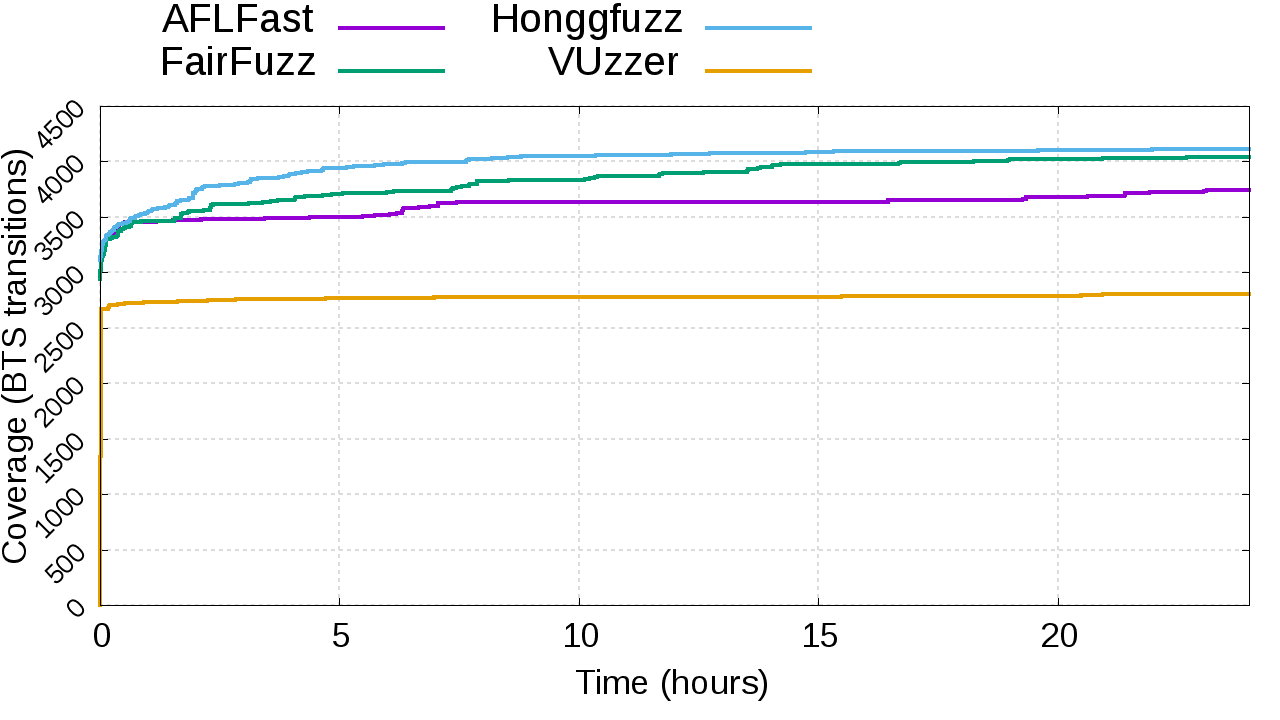
\includegraphics[width=\figwidth]{figures/mono-djpeg}
            }
            \subfloat[\objdump]{%
                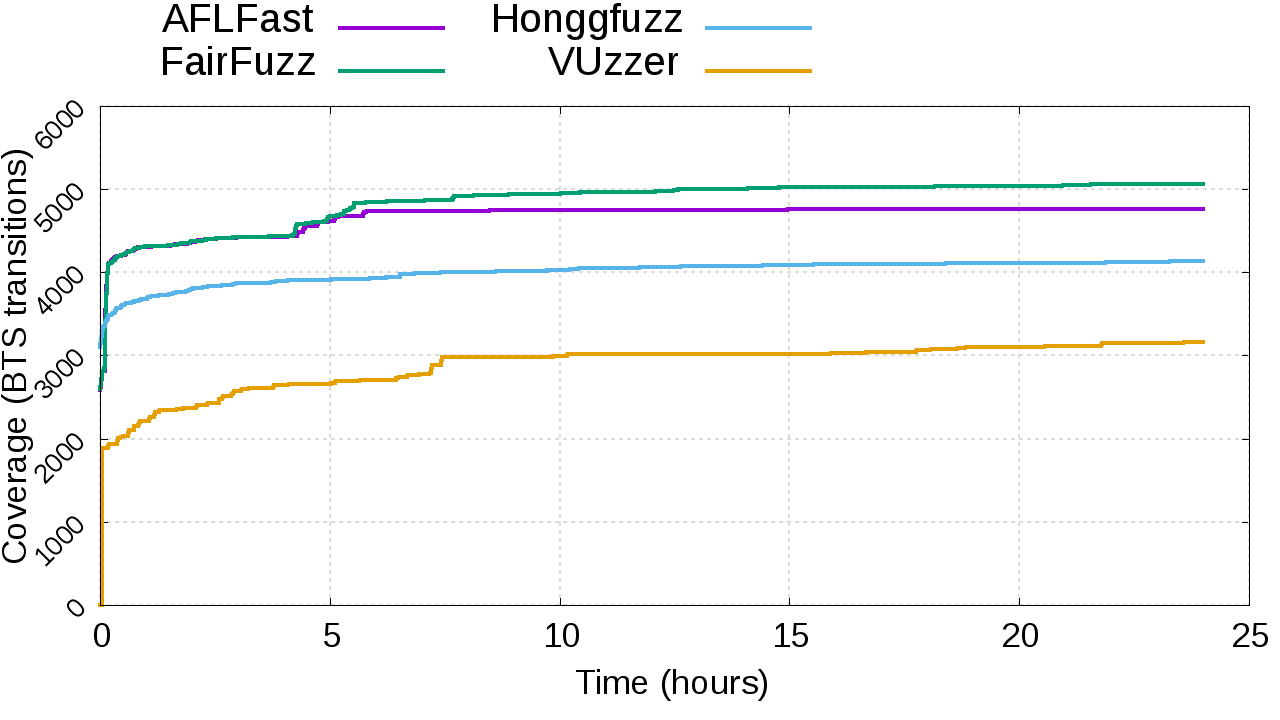
\includegraphics[width=\figwidth]{figures/mono-objdump}
            }
        \end{adjustbox}
        \begin{adjustbox}{center}
            \subfloat[\tiffpdf]{%
                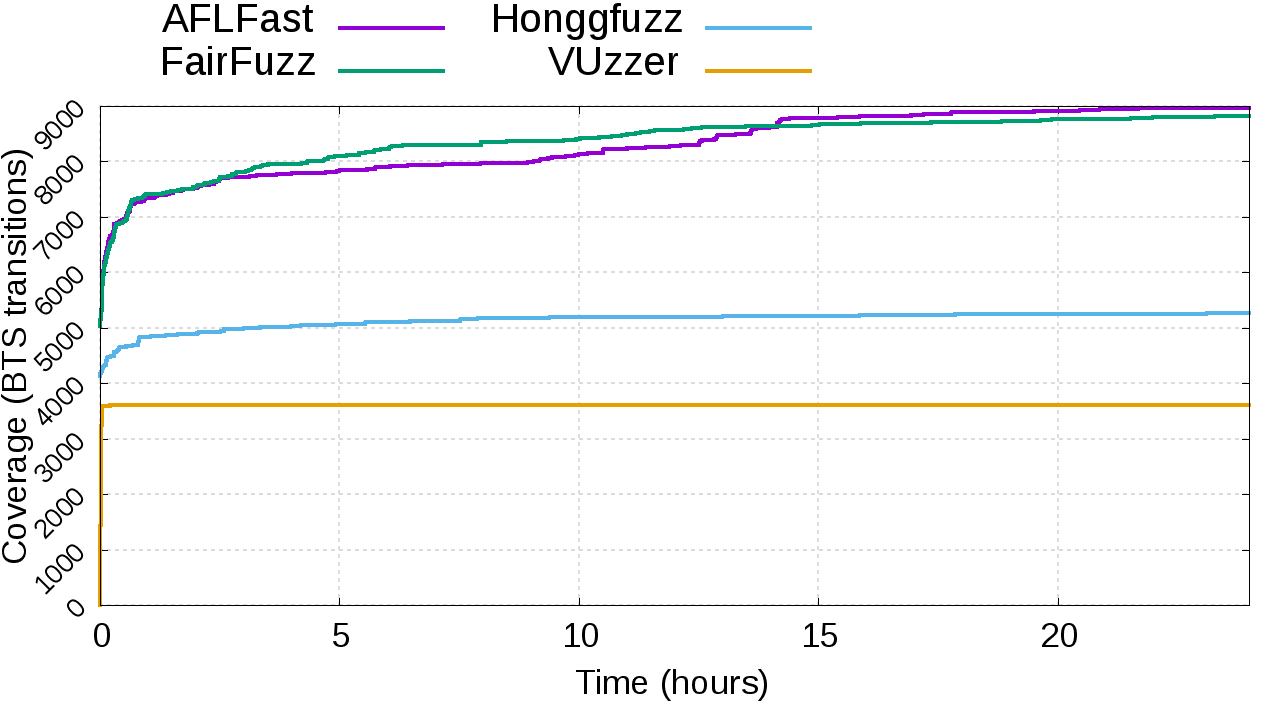
\includegraphics[width=\figwidth]{figures/mono-tiff2pdf}
            }
            \subfloat[\listswf]{%
                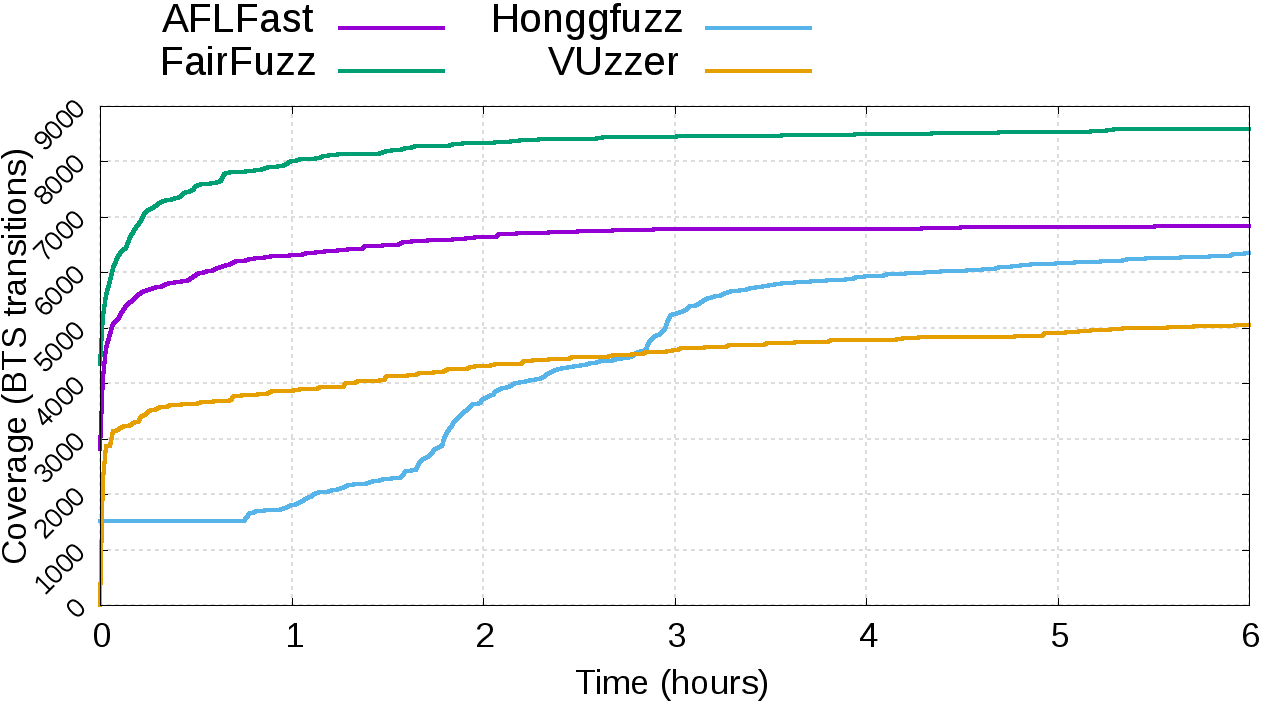
\includegraphics[width=\figwidth]{figures/mono-ming}
            }
        \end{adjustbox}
    \end{figure}
    \buttons{%
        \hyperlink{single-final<1>}{\beamergotobutton{Final means table}}
    }
    \script{%
        The figure shows the mean coverage over time for the 4 fuzzers on the 4
        targets. We see that in the first 3 cases, the curves are similar for
        the top 2 fuzzers; while for listswf, \fairfuzz\ seems to perform much
        better than the other.\\
        To have a better understanding, besides looking at the final means, I
        used a Bayesian estimation method to evaluate the difference of means
        between two fuzzers.
    }
\end{frame}

\begin{frame}[label=single-best]
    {Bayesian Estimation of Means}
    \renewcommand\figwidth{.32\textwidth}
    \setcounter{subfigure}{0}
    \begin{figure}
        \subfloat[\djpeg\\\honggfuzz\ vs.\ \fairfuzz]{%
            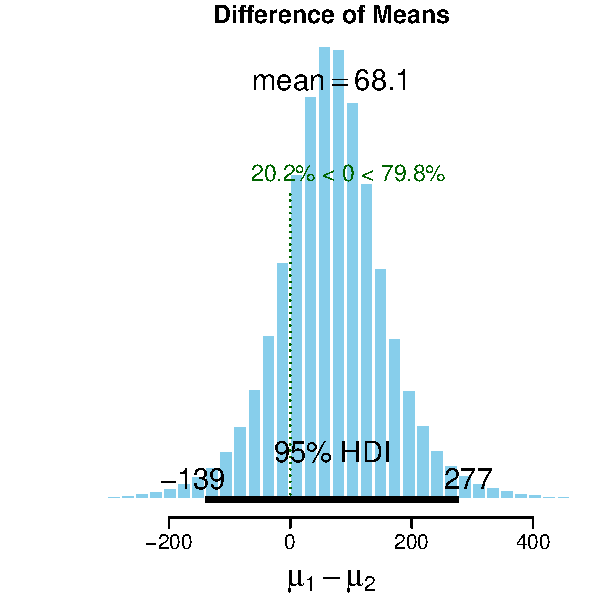
\includegraphics[width=\figwidth]{figures/cropped/djpeg-m-hongg-fair}
        }
        \subfloat[\objdump\\\fairfuzz\ vs.\ \aflfast]{%
            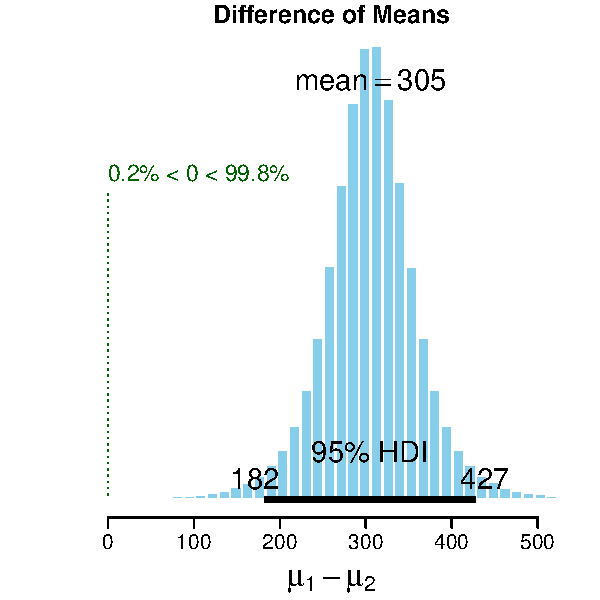
\includegraphics[width=\figwidth]{figures/cropped/objdump-m-fair-afl}
        }
        \subfloat[\tiffpdf\\\aflfast\ vs.\ \fairfuzz]{%
            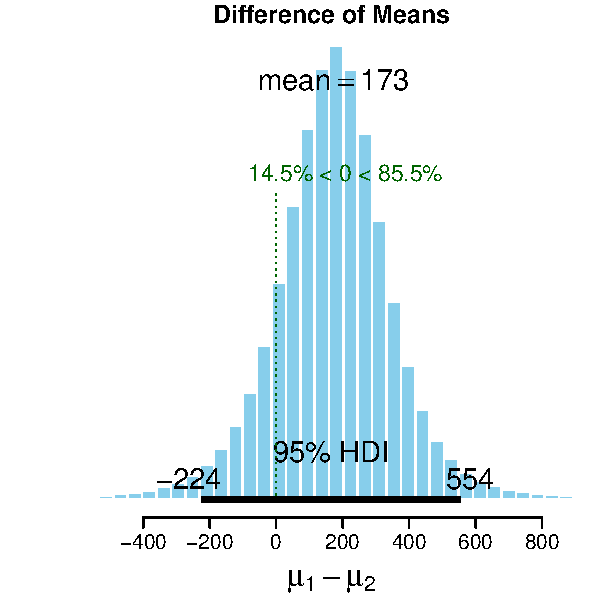
\includegraphics[width=\figwidth]{figures/cropped/tiff2pdf-m-afl-fair}
        }
    \end{figure}
    \begin{itemize}
        \item{} choose one for all $\longrightarrow$ \alert{\fairfuzz}
        \item{} chose one for each $\longrightarrow$ \alert{indecisive} for \djpeg~and \tiffpdf%
    \end{itemize}
    \buttons{%
        \hyperlink{single-final<1>}{\beamergotobutton{Final means table}}
    }
    \script{%
        \footnotesize
        The BEST method that I used models two groups of data as two separate
        $t$ distributions with priors on the means and standard deviations.
        Than, a sampling algorithm produces a number of parameter samples
        (\eg~two means, two standard deviations,\ldots) which are in accordance
        with the data. Each figure shows the difference of means at each sample
        for the first vs.\ second fuzzers in order of final mean coverage.

        To decide whether the difference in mean is high enough to declare a
        fuzzer better than the other, it is sufficient to look at the $95\%$
        High Density Interval: if it does not include zero, than one fuzzer is
        better than the other.
    }
\end{frame}

\begin{comment}
\begin{frame}
    {Do Fuzzers Uncover Different Transitions Sets?}
    \structure{Compare the fuzzer with highest coverage with union of fuzzers}
    \vspace{\baselineskip}
    \begin{table}
        \begin{tabular}{l c l c}
            \textbf{\sut} & \multicolumn{2}{c}{\textbf{best single}} & \textbf{union} \\
\bottomrule%
\djpeg& $4112.8 \pm 39.5476$ & \honggfuzz& \hicell$4157.2 \pm 40.0495$ \\
\objdump& $5067 \pm 62.6821$ & \fairfuzz& \hicell$5404.6 \pm 38.1997$ \\
\tiffpdf& $8971.2 \pm 152.8626$ & \aflfast& \hicell$9695 \pm 129.7239$ \\
\listswf& $8586.8 \pm 87.7451$ & \fairfuzz& \hicell$8916.6 \pm 83.8365$


        \end{tabular}
    \end{table}
    \vspace{\baselineskip}
    \structure{Bayesian estimation agrees, except for \djpeg}
\end{frame}
\end{comment}

\subsection{Cooperative Fuzzing Evaluation}

\begin{frame}
    {Evaluating the Effect of Cooperation}
    \begin{block}{Cooperative strategies}
        \begin{itemize}
            \item{} score is number of newly discovered BTS transitions
            \item{} single highest winner strategy
            \item{} multiple positive-scored winners strategy
        \end{itemize}
    \end{block}
    \script<1>{%
        I'm going to present results on two coop.\ strategies that use the same
        scoring function (number of newly discovered BTS transitions) and change
        how they select winners: one selects a single winner with the highest
        score; the other selects all fuzzers which report a score greater than
        zero.
    }
    \begin{block}<2->{Experiment design}
        \begin{enumerate}
            \item{} run CFF with selected strategy for 6 hours
            \item{} drivers log coverage for respective fuzzer
            \item{} compare mean coverage over 5 runs against union of fuzzers
        \end{enumerate}
    \end{block}
    \script<2>{%
        Experiments are conducted on the same 4 targets as before, except that
        they last 6 hours instead of 24. Coverage is collected during normal
        operation of the system and the result from each coop.\ strategy is
        compared with the union of BTS transitions discovered by single fuzzers.
        In other words, the union is a post processing step on the data obtained
        during our previous evaluation, limited to the 6th hour mark.
    }
\end{frame}

\begin{frame}[label=coop-time]
    {Mean Coverage Over Time}
    \renewcommand\figwidth{.42\textwidth}
    \setcounter{subfigure}{0}
    \vspace{-\baselineskip}
    \begin{figure}[h]
        \begin{adjustbox}{center}
            \subfloat[\djpeg]{%
                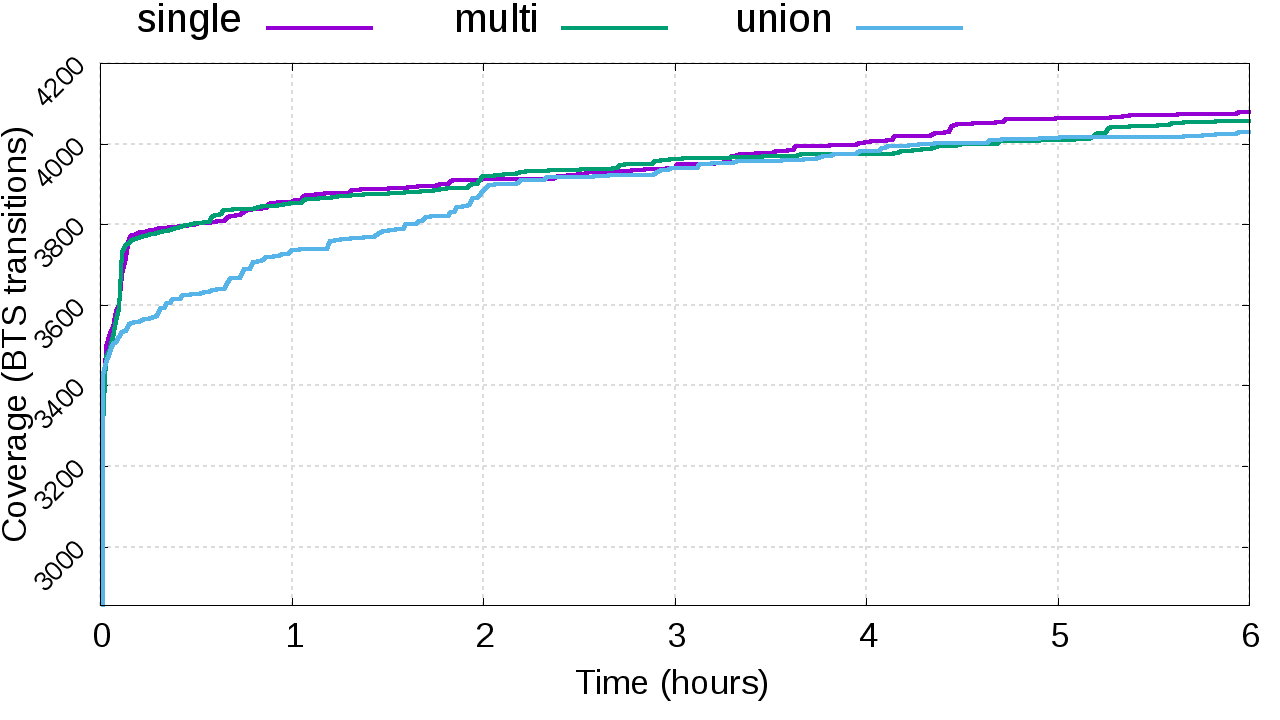
\includegraphics[width=\figwidth]{figures/vs-djpeg}
            }
            \subfloat[\objdump]{%
                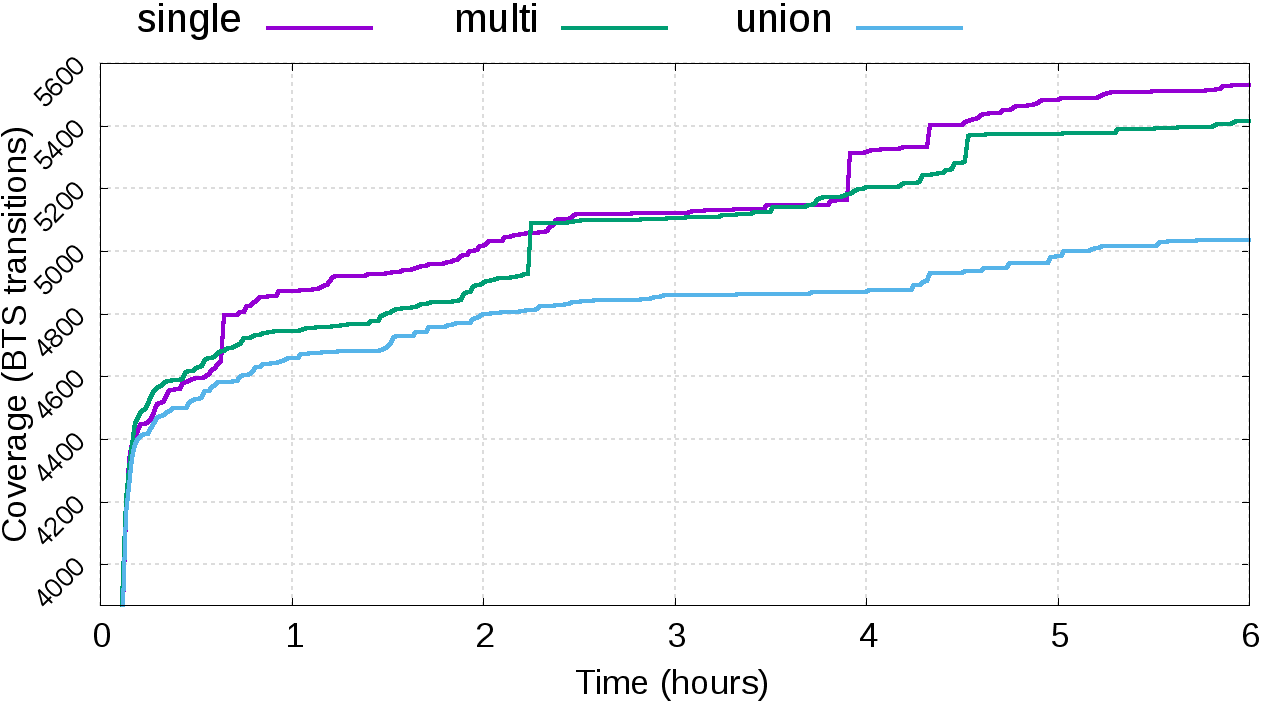
\includegraphics[width=\figwidth]{figures/vs-objdump}
            }
        \end{adjustbox}
        \begin{adjustbox}{center}
            \subfloat[\tiffpdf]{%
                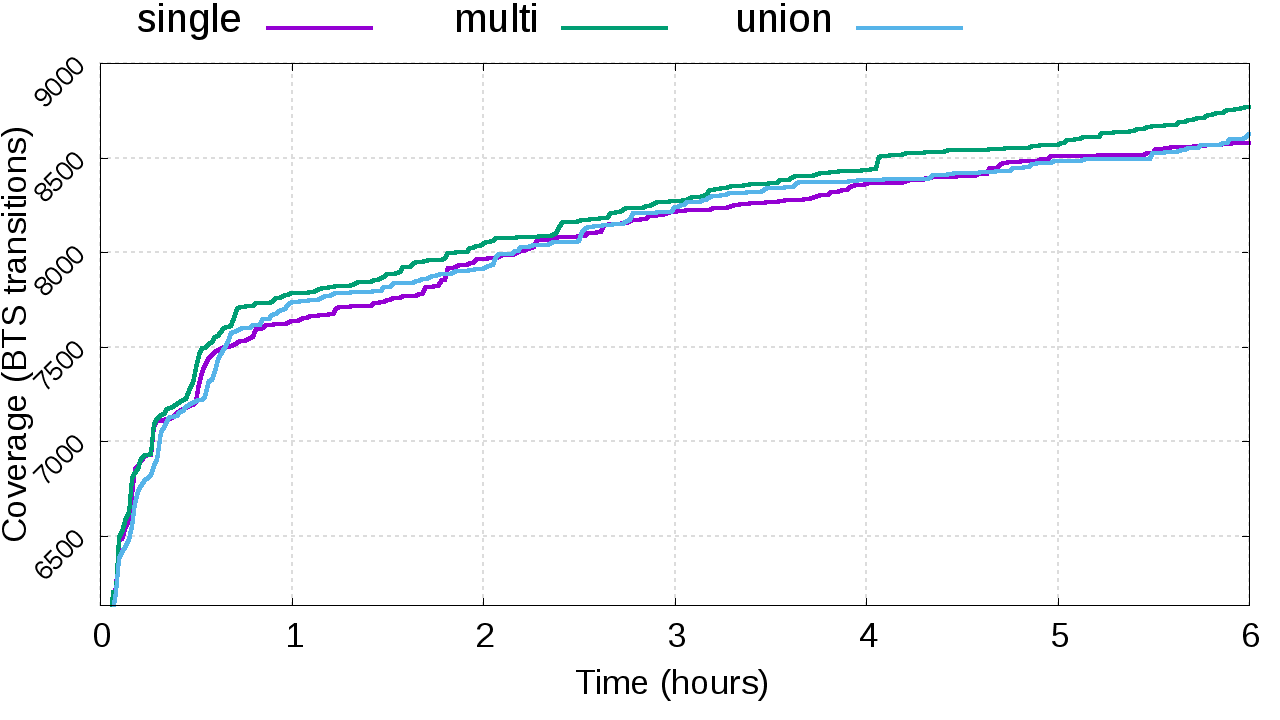
\includegraphics[width=\figwidth]{figures/vs-tiff2pdf}
            }
            \subfloat[\listswf]{%
                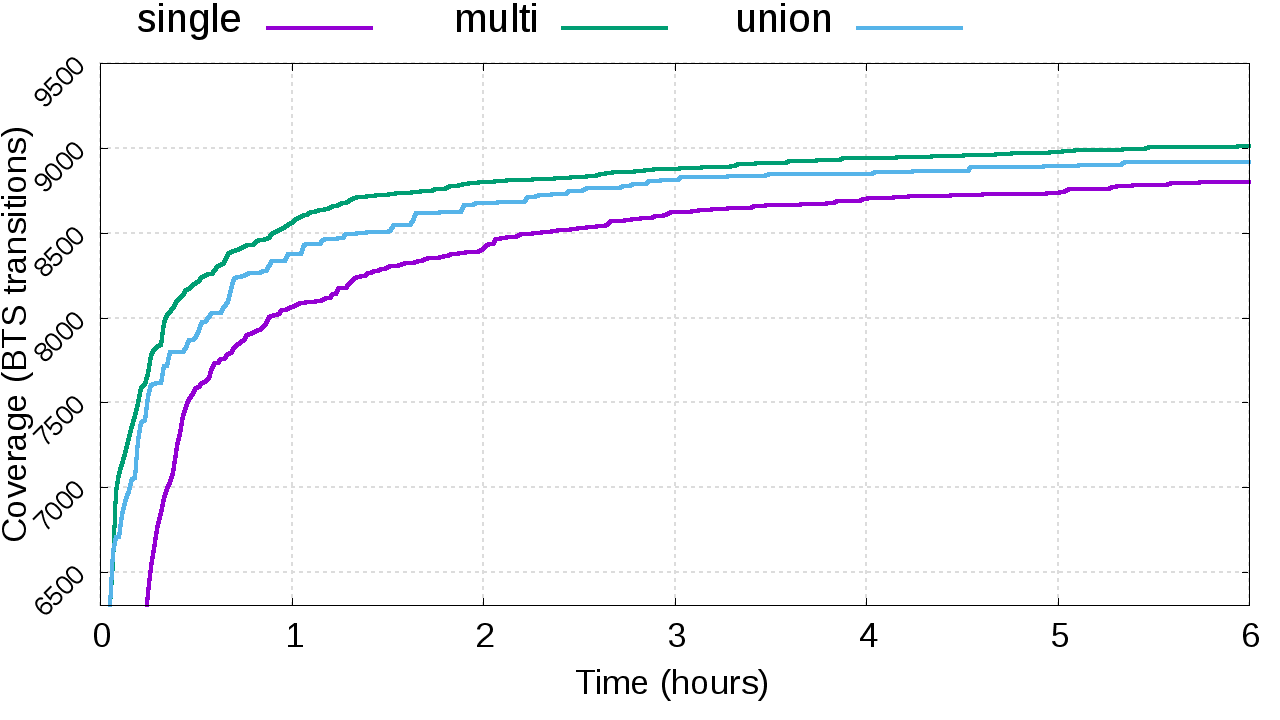
\includegraphics[width=\figwidth]{figures/vs-ming}
            }
        \end{adjustbox}
    \end{figure}
    \buttons{%
        \hyperlink{coop-final<1>}{\beamergotobutton{Final means table}}
    }
    \script{%
        The figure shows the mean coverage over time for the two coop.\
        strategies and the union of fuzzers. In particular the multi.\ strat.\
        outperforms the union for all targets, while the single strat.\ performs
        the best for the first two targets and the worst for the last two.
    }
\end{frame}

\begin{frame}[label=coop-best]
    {Bayesian Estimation of Means}
    \renewcommand\figwidth{.28\textwidth}
    \setcounter{subfigure}{0}
    \begin{figure}
        \begin{adjustbox}{center}
            \subfloat[\djpeg\\single vs.\ union]{%
                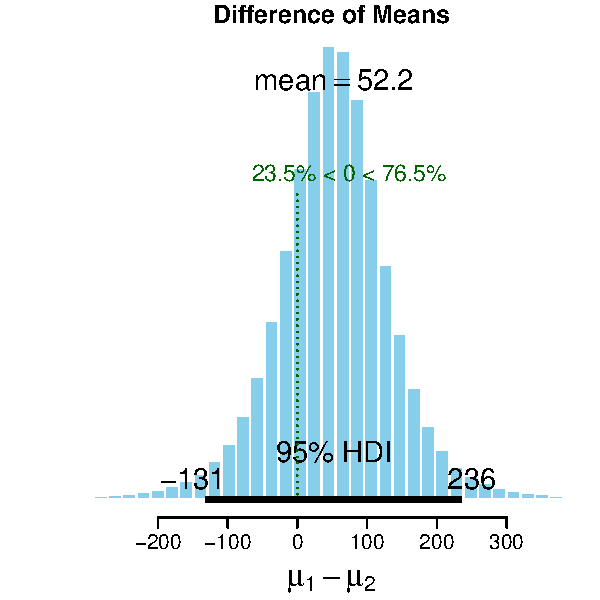
\includegraphics[width=\figwidth]{figures/cropped/djpeg-m-single-uni}
            }\hspace{-.05\textwidth}
            \subfloat[\objdump\\single vs.\ union]{%
                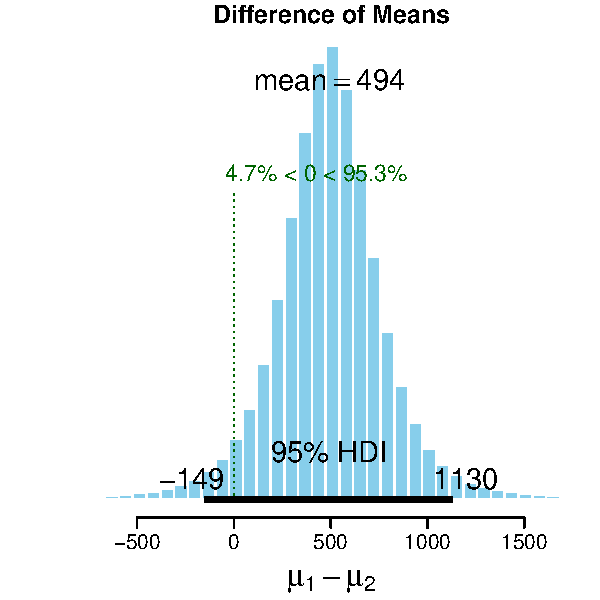
\includegraphics[width=\figwidth]{figures/cropped/objdump-m-single-uni}
            }\hspace{-.05\textwidth}
            \subfloat[\tiffpdf\\multi vs.\ union]{%
                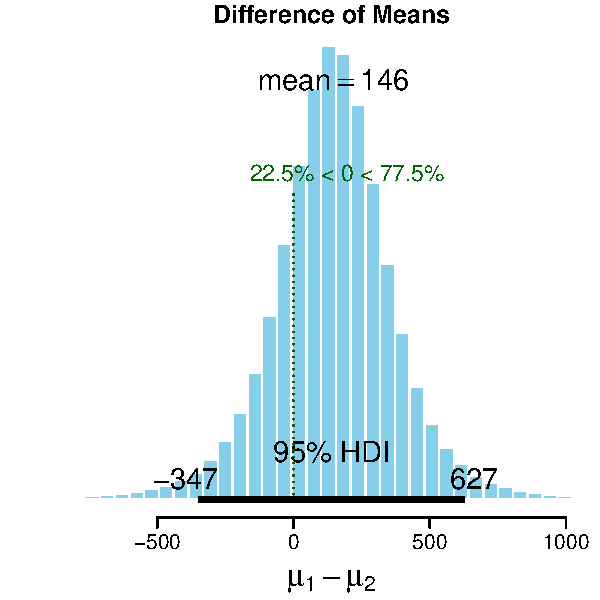
\includegraphics[width=\figwidth]{figures/cropped/tiff2pdf-m-multi-uni}
            }\hspace{-.05\textwidth}
            \subfloat[\listswf\\multi vs.\ union]{%
                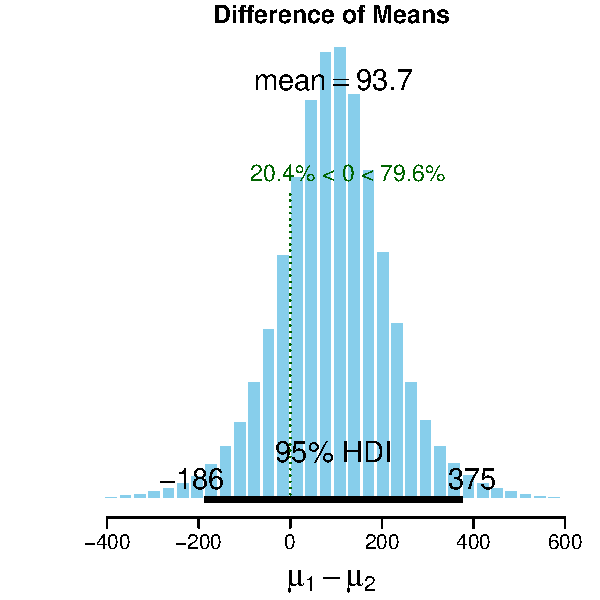
\includegraphics[width=\figwidth]{figures/cropped/ming-m-multi-uni}
            }
        \end{adjustbox}
    \end{figure}
    \begin{itemize}
        \item{} \djpeg, \tiffpdf~and \listswf~$\longrightarrow$ \alert{indecisive}
        \item{} \objdump~$\longrightarrow$ \parbox{.7\textwidth}{%
                \alert{indecisive} but not by much\\
                multi vs.\ union $96.7\%$ of HDI is $> 0$}
    \end{itemize}
    \buttons{%
        \vspace{.5\baselineskip}
        \hyperlink{coop-final<1>}{\beamergotobutton{Final means table}}
    }
    \script{%
        Again, I used BEST to mutually compare the final means for the different
        experiments. The figures show the result for the strat.\ with highest
        final mean coverage vs.\ the union of fuzzers.

        Unfortunately, by looking at the $95\%$ HDI, we cannot say with high
        credibility that any of the coop.\ strategies outperforms the union of
        fuzzers. In particular for 3 targets, roughly $77\%$ of HDI is above
        zero and for objdump $95.3\%$ is.
    }
\end{frame}

\subsection{Crash Analysis and Known Vulnerabilities}

\begin{frame}
    {Unique Crash Analysis}
    \begin{block}<1->{Obtaining unique crashes}
        \begin{enumerate}
            \item{} fuzzers collect crashes in folder
            \item{} re-execute target with input and run \texttt{exploitable} (stack hash)
            \item{} stack hash and elapsed time for 5 runs in single file
        \end{enumerate}
    \end{block}
    \script<1>{%
        To obtain unique crashes, which are inputs that cause a crash through a
        unique path, every crashing input stored by fuzzers is fed to the
        target. This is done to validate the crash and get its stack hash, which
        is the hash of the last calls on the stack before the crash. The stack
        hashes and relative elapsed time from 5 runs are accumulated into a
        single file and processed.
    }
    \uncover<2->{%
        \vspace{\baselineskip}
        \begin{table}
            \begin{tabular}{l c c c c}
                & \textbf{Unique crashes} & \textbf{Vs.\ single} &
\textbf{Vs.\ multi} & \textbf{Vs.\ union} \\
\bottomrule%
\textbf{union} & $75$ & $21$ & $13$ & \\
\hline%
\textbf{multi} & $98$ & $44$ & & $36$ \\
\hline%
\textbf{single} & $63$ & & $9$ & $9$


            \end{tabular}
            \caption{Crashes in \listswf}
        \end{table}
    }
    \script<2>{%
        Unfortunately crashes were found only on listswf. The table shows the
        number of distinct unique crashes and the number of unique crashes that
        are found by one fuzzer and not by another. In particular the multi
        strat.\ finds $30\%$ more distinct unique crashes than the union and
        more crashes that the union doesn't find.
    }
\end{frame}

\begin{frame}
    {Unique Crashes Over Time --- \listswf}
    \renewcommand\figwidth{.32\textwidth}
    \setcounter{subfigure}{0}
    \captionsetup[subfigure]{margin=3pt}
    \begin{figure}
        \subfloat[Cumulative]{%
            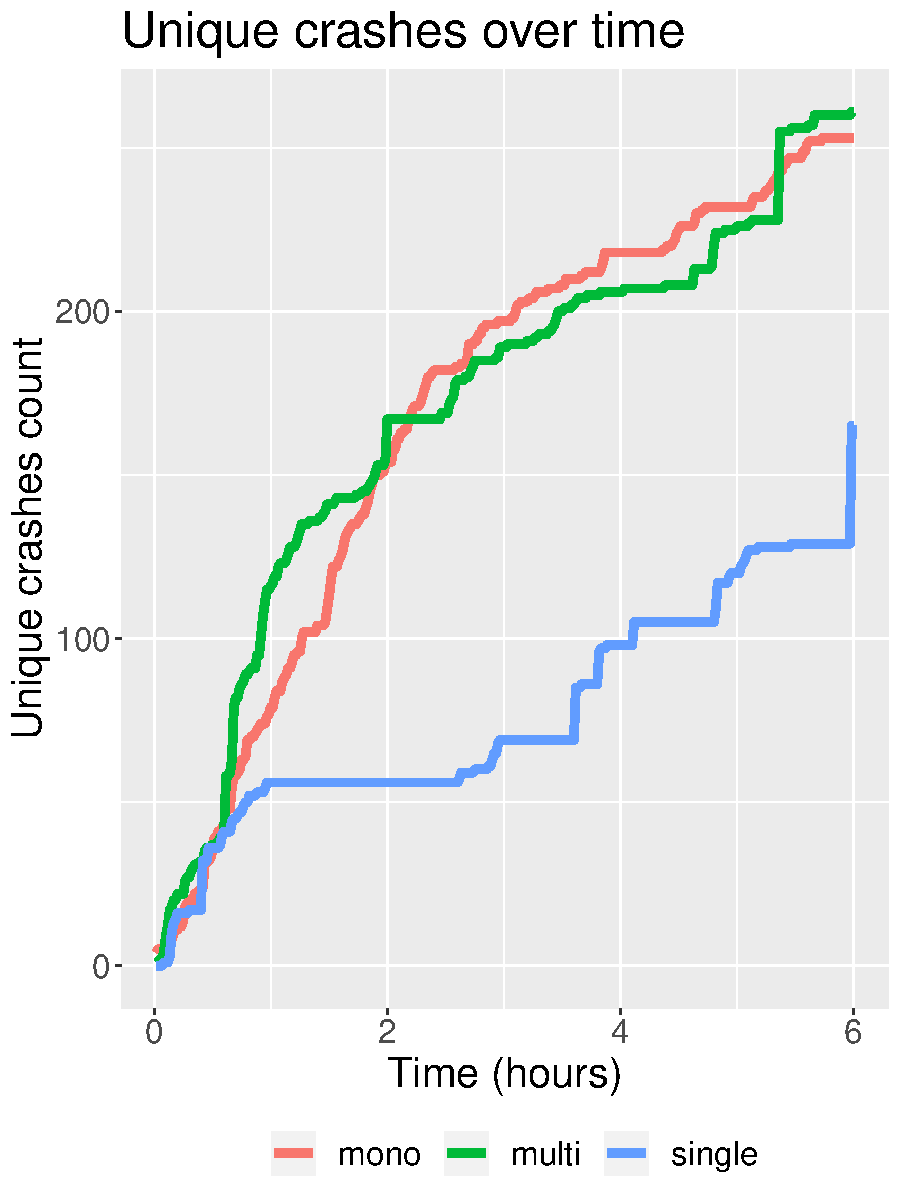
\includegraphics[width=\figwidth]{figures/cropped/crashes-count-all}
        }
        \subfloat[Density]{%
            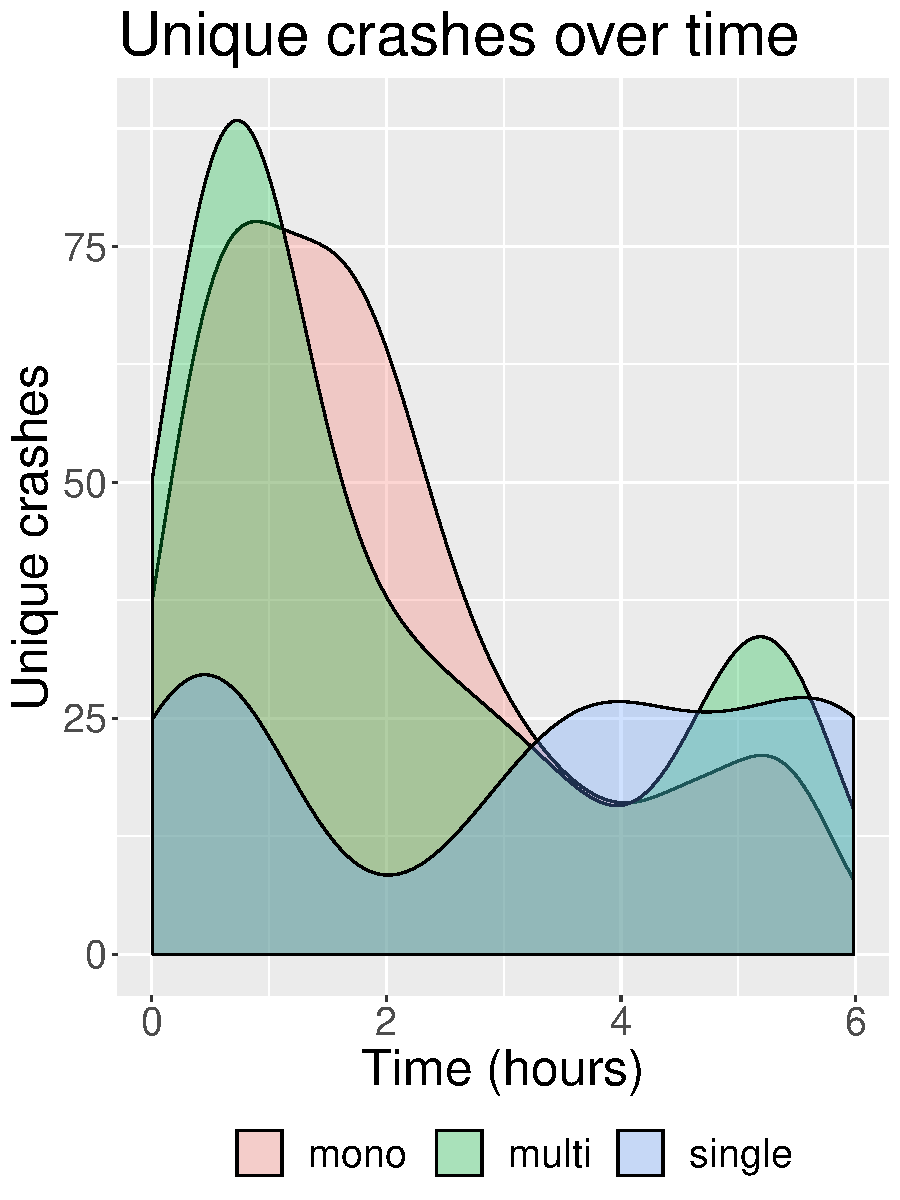
\includegraphics[width=\figwidth]{figures/cropped/crashes-all}
        }
        \subfloat[Uncommon density]{%
            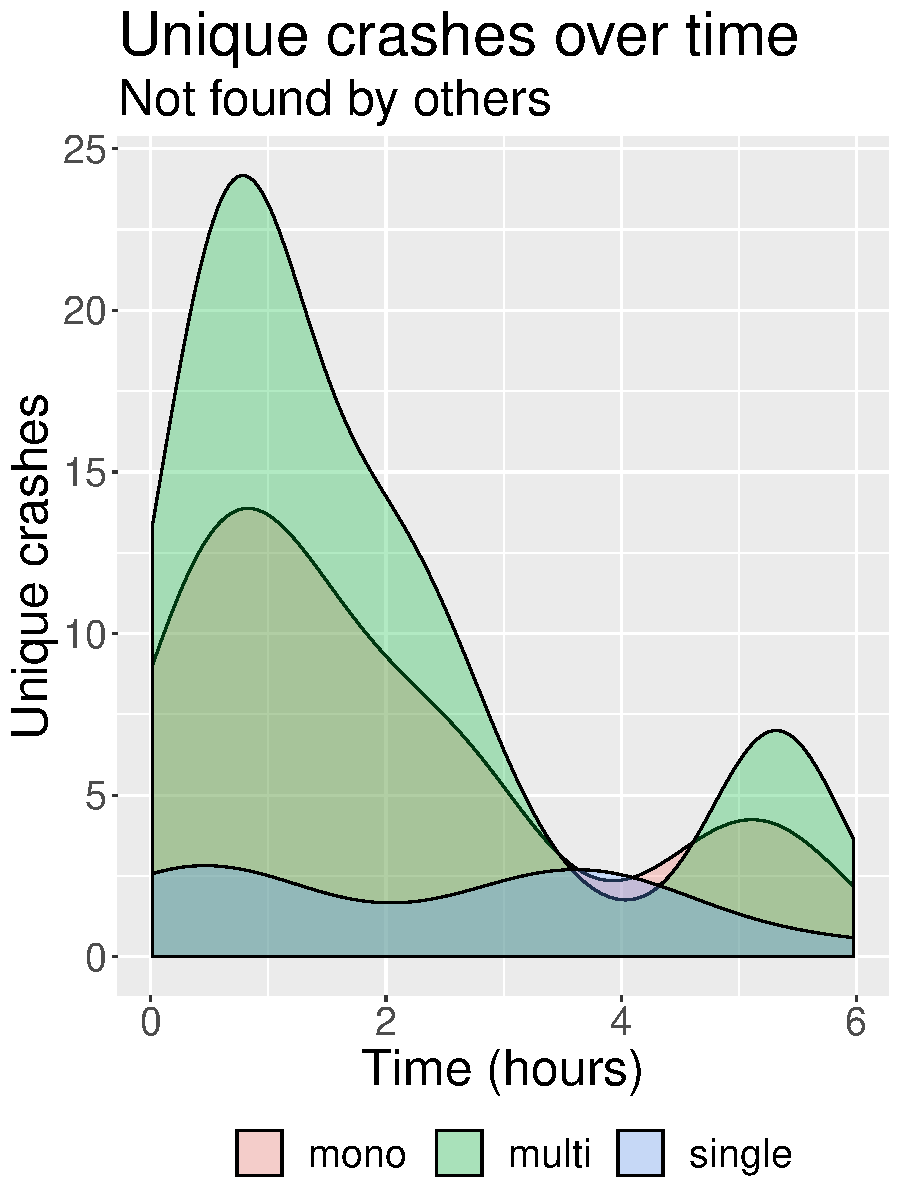
\includegraphics[width=\figwidth]{figures/cropped/crashes-not-intersect}
        }
    \end{figure}
    \script{%
        The figure on the left shows the cumulative count of crashes over time,
        across the 5 runs; we see that the curves for the multi strategy and the
        union of fuzzers are similar. The figure in the middle shows the density
        of crashes over time: in particular we note that the multi strategy
        finds the most crashes at the beginning and at the very end of the runs.
        This is also true for the union of fuzzers, but with less amplitude on
        the peaks. The same behaviour is visible in the last figure where only
        crashes not found by the others are considered.
    }
\end{frame}

\begin{frame}
    {Known Vulnerabilities --- \listswf}
    \begin{columns}
        \begin{column}{.66\textwidth}
            \renewcommand\figwidth{.33\textwidth}
            \vspace{-20pt}
            \begin{figure}
                \subfloat{%
                    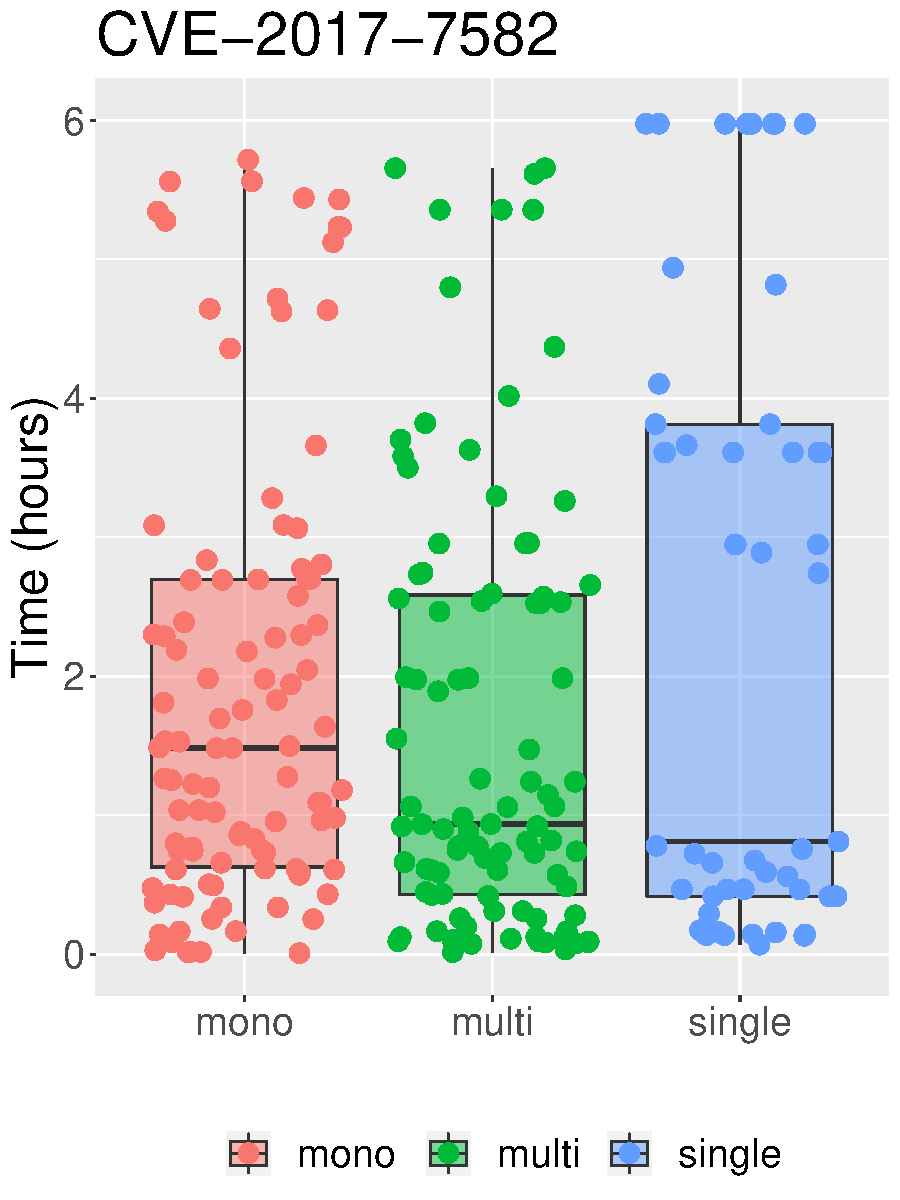
\includegraphics[width=\figwidth]{figures/cropped/cve-2017-7582}
                }
                \subfloat{%
                    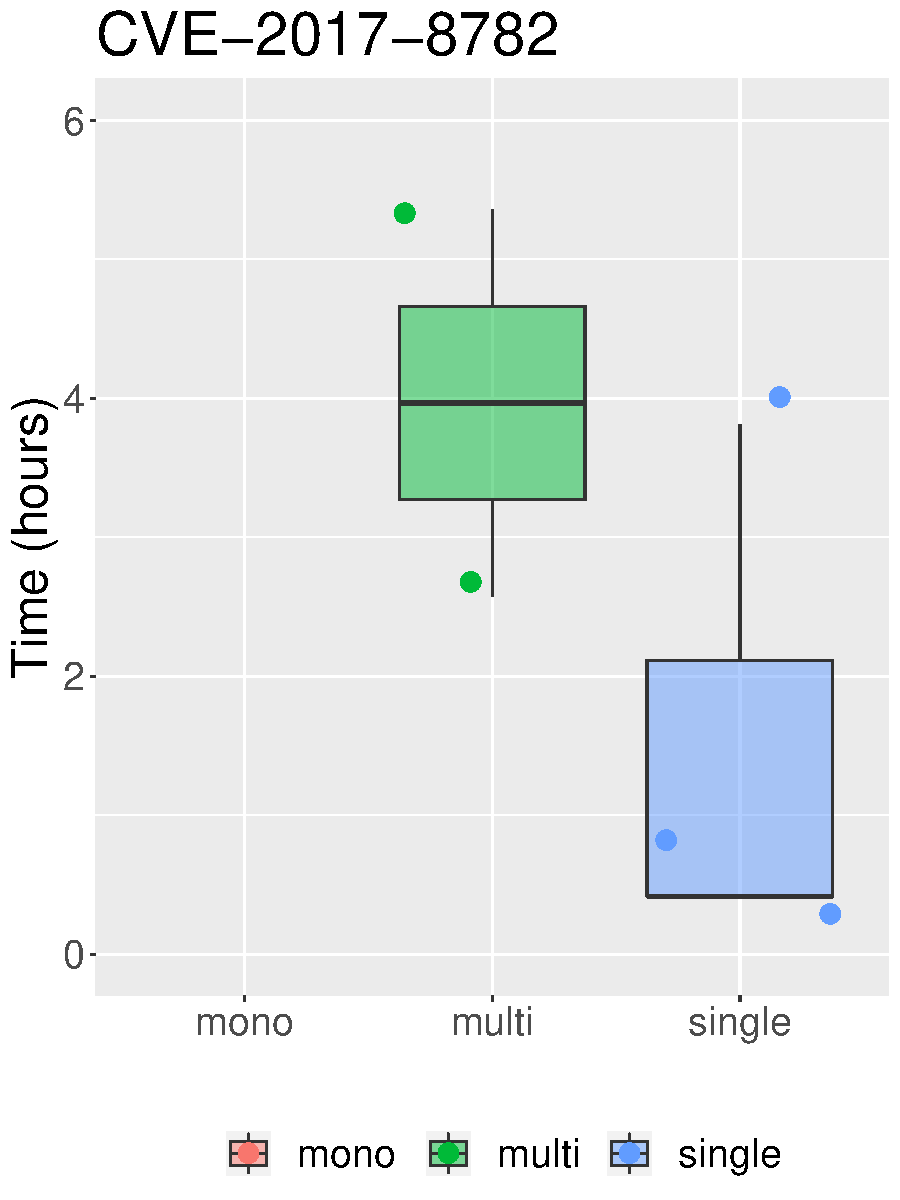
\includegraphics[width=\figwidth]{figures/cropped/cve-2017-8782}
                }
                \subfloat{%
                    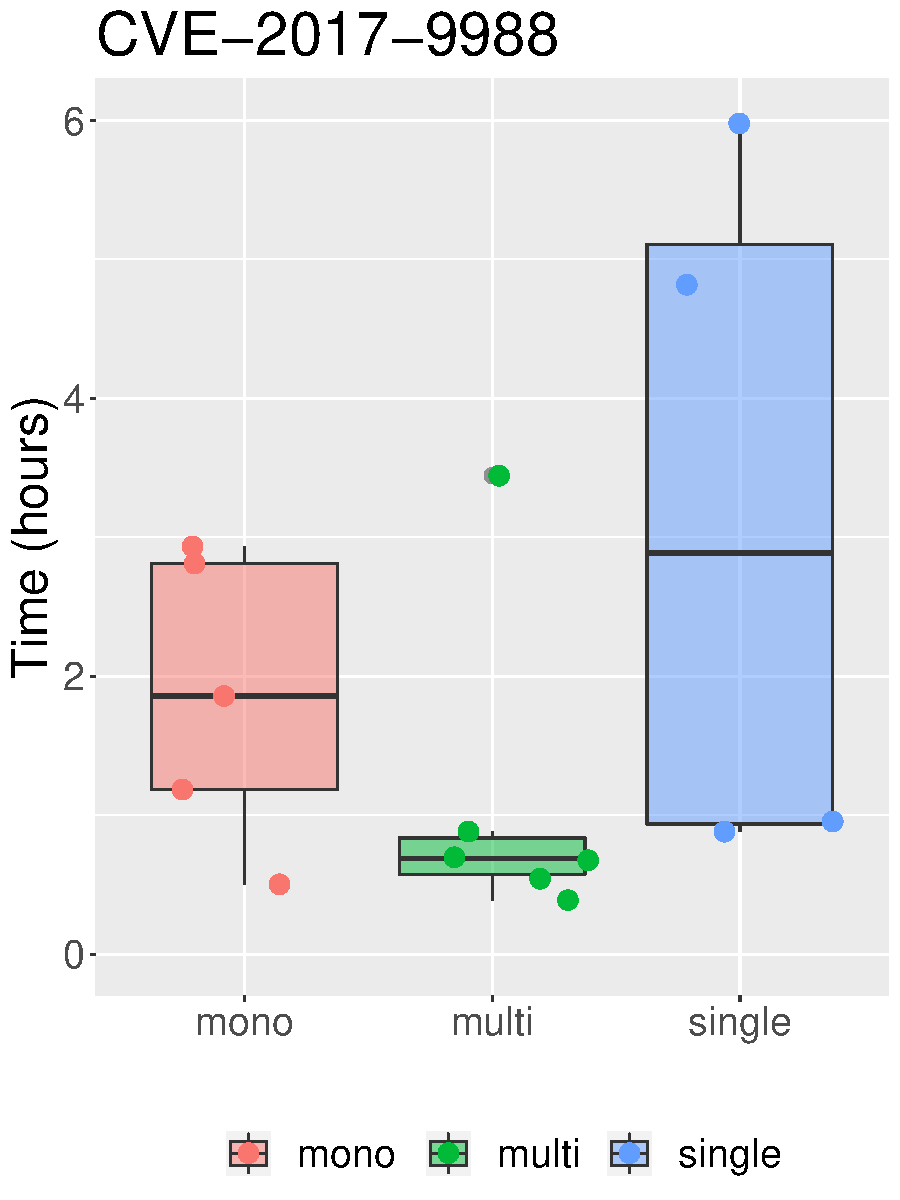
\includegraphics[width=\figwidth]{figures/cropped/cve-2017-9988}
                }
                \vspace{-8pt}
                \subfloat{%
                    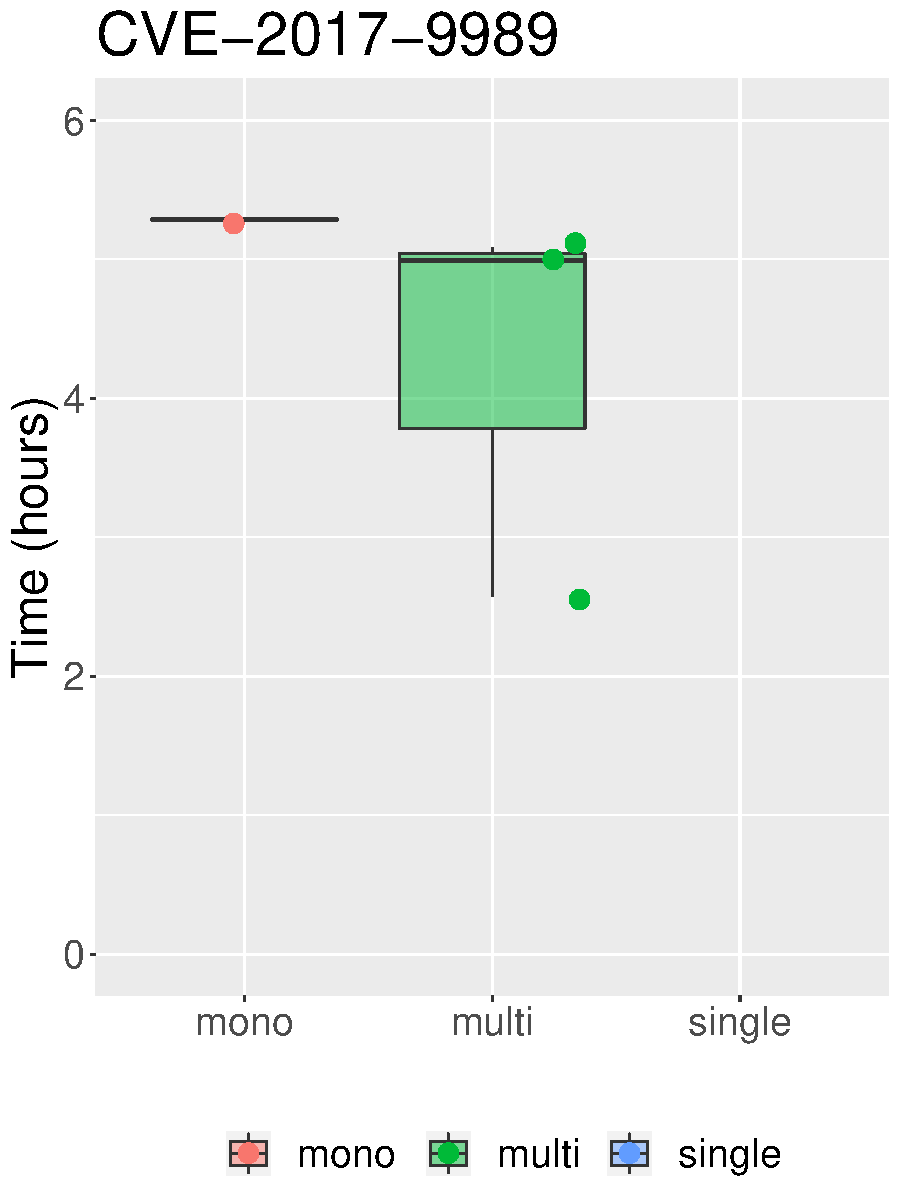
\includegraphics[width=\figwidth]{figures/cropped/cve-2017-9989}
                }
                \subfloat{%
                    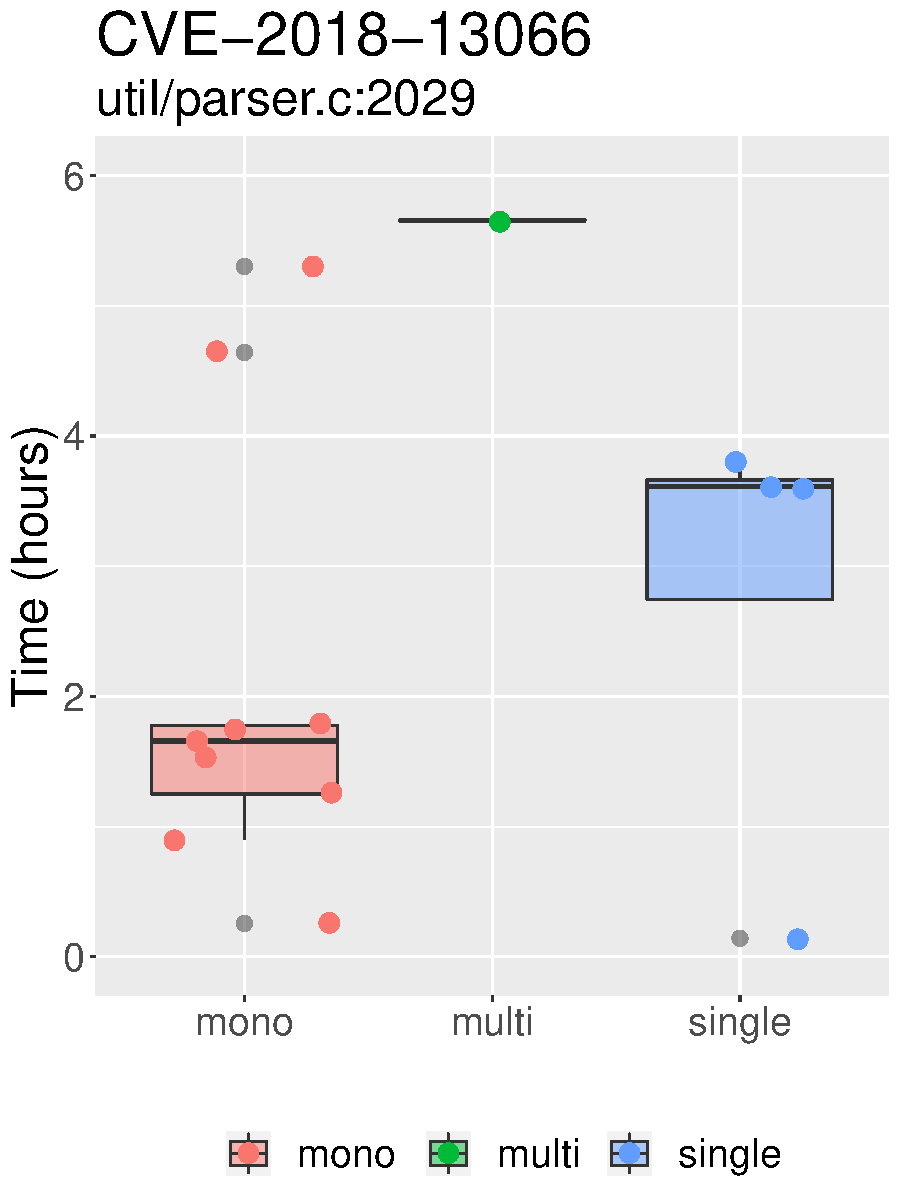
\includegraphics[width=\figwidth]{figures/cropped/cve-2018-13066-parser-2029}
                }
                \subfloat{%
                    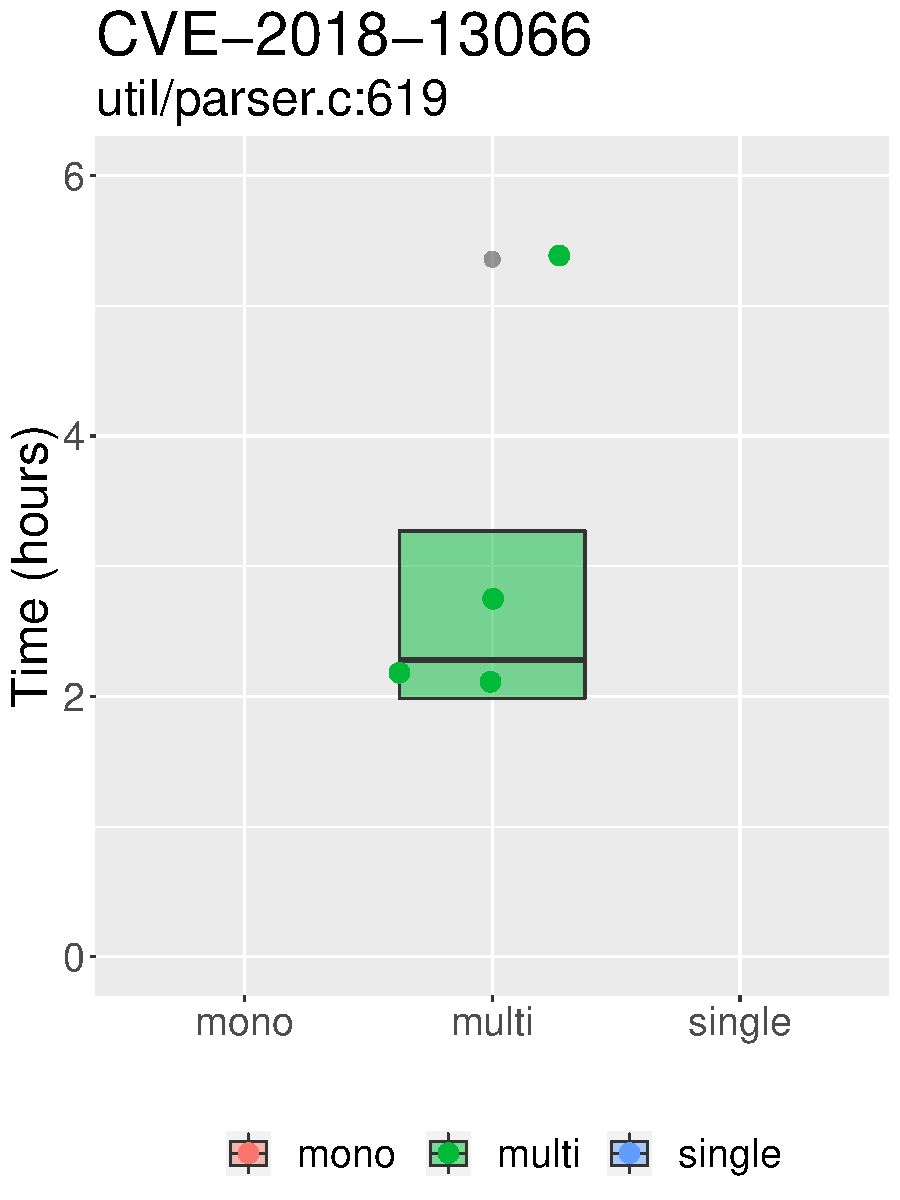
\includegraphics[width=\figwidth]{figures/cropped/cve-2018-13066-parser-619}
                }
            \end{figure}
        \end{column}
        \begin{column}{.33\textwidth}
            \begin{itemize}
                \item{} over 25 bugs,\\6 linked to a CVE
                \item{} multi winners\\finds all CVE\\found by union
                \item{} all but one found earlier than union
                \item{} finds two CVE\\not found by union
            \end{itemize}
        \end{column}
    \end{columns}
    \script{%
        To conclude the analysis, I manually investigated unique crashes to try
        to group them by causing bug, as more unique crashes may be caused by
        the same bug. Of the over 25 bugs I was able to link 6 to a CVE
        identifier. Each of the figures shows a boxplot of the elapsed time to
        find a crash that triggers the specific vulnerability. In particular the
        multi strategy finds all vulnerabilities found by the union of fuzzers
        and all but one are found earlier. Moreover it finds two vulnerabilities
        that the union doesn't find.
    }
\end{frame}

\section{Discussion and Conclusion}

\begin{frame}
    \tableofcontents[currentsection]
\end{frame}

\subsection*{Discussion}

\begin{frame}
    {Discussion}
    \begin{itemize}
        \item{} \structure{is there a best fuzzer?}
            \begin{itemize}
                \item{} on average yes, but need more than 4 targets
                \item{} indecisive for some targets, need more than 5 runs
            \end{itemize}
        \item{} \structure{does cooperation increase coverage?}
            \begin{itemize}
                \item{} observed means suggest yes (on average better more
                    communication)
                \item{} $95\%$ HDI difference of means never excludes zero
                \item{} nonetheless promising results, need more data
            \end{itemize}
        \item{} \structure{what is the effect of cooperation on crashes?}
            \begin{itemize}
                \item{} unfortunately data only on one target
                \item{} multi finds $30\%$ more distinct unique crashes than union
                \item{} multi finds more unique crashes not found by other
                \item{} multi has strongly bimodal crash density
                \item{} multi finds all CVE union finds (+2 more), earlier
            \end{itemize}
    \end{itemize}
\end{frame}

\subsection*{Conclusion}

\begin{frame}
    {Conclusion}
    \begin{block}{Summary}
        \begin{itemize}
            \item{} design of Cooperative Fuzzing Framework
            \item{} prototype implementation of CFF
            \item{} evaluation of single fuzzers and cooperation
        \end{itemize}
    \end{block}
    \begin{block}{Future work}
        \begin{itemize}
            \item{} more experiments (targets, runs)
            \item{} more fuzzers (purely black box or white box)
            \item{} more complex strategies / scoring functions
        \end{itemize}
    \end{block}
\end{frame}

\appendix

\section{\appendixname}

\setbeamertemplate{page number in head/foot}{}

\begin{frame}[noframenumbering]
    \tableofcontents[]
\end{frame}

\AtBeginSubsection[]{}

\subsection{Bayesian Estimation}

\begin{frame}[noframenumbering,label=best]
    {Bayesian Estimation Supersedes the $t$ Test}
    \begin{center}
        \begin{tikzpicture}[
            box/.style = {rectangle,
                color = lightgray,
                text = black,
                text width = 2cm,
                align = center},
            node distance=.3cm]
            \node[box] (y1) {$y_{1i}$};
            \node[box,xshift=4cm] (y2) {$y_{2i}$};
            \node[box,above=of y1] (t1) {\tdist};
            \node[box,above=of y2] (t2) {\tdist};
            \node[box,above=of y1,yshift=.5cm] (mu1) {$\mu_1$};
            \node[box,above=of y2,yshift=.5cm] (mu2) {$\mu_2$};
            \node[box,above=of y1.west,yshift=.4cm] (sig1) {$\sigma_1$};
            \node[box,above=of y2.east,yshift=.4cm] (sig2) {$\sigma_2$};
            \node[box,above=of y1.north east,yshift=.4cm] (nu1) {$\nu$};
            \node[box,above=of y2.north west,yshift=.4cm] (nu2) {$\nu$};
            \nodeshifexpdist{nu}{above=of t1,yshift=-.8cm,xshift=2cm}
            \nodenormdist{norm1}{above=of t1}
            \nodenormdist{norm2}{above=of t2}
            \nodeunidist{uni1}{above=of t1.north west,yshift=-.8cm,xshift=-.6cm}
            \nodeunidist{uni2}{above=of t2.north east,yshift=-.8cm,xshift=.6cm}
            \draw[->] (t1) -- (y1);
            \draw[->] (t2) -- (y2);
            \draw[->] (norm1) -- node[left] {$\sim$} (mu1);
            \draw[->] (norm2) -- node[left] {$\sim$} (mu2);
            \draw[->] (uni1) -- node[left] {$\sim$} (sig1);
            \draw[->] (uni2) -- node[right] {$\sim$} (sig2);
            \draw[->] (nu) -- node[left] {$\sim$} (nu1);
            \draw[->] (nu) -- node[right] {$\sim$} (nu2);
        \end{tikzpicture}
    \end{center}
    \begin{itemize}
        \item{} models two groups of observations as two $t$ distributions\\
            parameters are $\langle\mu_1,\sigma_1,\mu_2,\sigma_2,\nu\rangle$
        \item{} broad priors with parameters scaled on data
        \item{} Markov Chain Monte Carlo sampling\\
            (\eg~$\mu_1-\mu_2$ computed at each sample)
    \end{itemize}
\end{frame}

\subsection{Mean Coverage Tables}

\begin{frame}[noframenumbering,label=single-final]
    {Final Mean Coverage for Single Fuzzers}
    \begin{table}
        \scriptsize
        \begin{tabular}{l*{4}c}
            \textbf{\sut} & \textbf{\aflfast} & \textbf{\fairfuzz} &
    \textbf{\honggfuzz} & \textbf{\vuzzer} \\
\bottomrule%
\djpeg& $3739.4 \pm 113.831$ & $4043.2 \pm 103.838$ &
    \hicell$4112.8 \pm 39.5483$ & $2801 \pm 53.5514$ \\
\objdump& $4762.6 \pm 23.3693$ & \hicell$5067 \pm 62.6832$ &
    $4132.4 \pm 104.8$ & $3162.2 \pm 138.462$ \\
\tiffpdf& \hicell$8971.2 \pm 152.865$ & $8813.8 \pm 146.756$ &
    $5260.2 \pm 148.591$ & $3616 \pm 34.6427$ \\
\listswf& $6831.6 \pm 2615.24$ & \hicell$8586.8 \pm 87.7467$ &
    $6345.6 \pm 2358.52$ & $5048.2 \pm 90.3928$


        \end{tabular}
    \end{table}
    \buttons{%
        \vspace{2\baselineskip}
        \hyperlink{single-time<1>}{\beamerreturnbutton{Coverage over time}}
        \hyperlink{single-best<1>}{\beamerreturnbutton{Bayesian estimation}}
    }
\end{frame}

\begin{frame}[noframenumbering,label=coop-final]
    {Final Mean Coverage for Cooperative Fuzzing}
    \begin{table}
        \begin{tabular}{l c c c}
            \textbf{\sut} & \textbf{multi} & \textbf{single} & \textbf{union} \\
\bottomrule%
\djpeg& $4056.4 \pm 76.9499$ & \hicell$4078.4 \pm 85.6738$ & $4028.6 \pm 47.7396$ \\
\objdump& $5414.6 \pm 224.121$ & \hicell$5529.6 \pm 338.651$ & $5035.6 \pm 54.5944$ \\
\tiffpdf& \hicell$8765.6 \pm 183.682$ & $8577.6 \pm 99.2457$ & $8623.2 \pm 183.399$ \\
\listswf& \hicell$9008.4 \pm 122.81$ & $8801.4 \pm 96.4045$ & $8916.6 \pm 83.8381$


        \end{tabular}
    \end{table}
    \buttons{%
        \vspace{2\baselineskip}
        \hyperlink{coop-time<1>}{\beamerreturnbutton{Coverage over time}}
        \hyperlink{coop-best<1>}{\beamerreturnbutton{Bayesian estimation}}
    }
\end{frame}

\subsection{Overhead Evaluation}

\begin{frame}[noframenumbering]
    {Overhead of CFF}
    \begin{block}{Sources of overhead}
        \begin{itemize}
            \item{} fuzzers synchronize with file system
            \item{} drivers:
                \begin{itemize}
                    \item{} get BTS trace for every ``interesting'' input
                    \item{} reply to metric requests (BTS diff)
                    \item{} receives new input from master (copy input, add coverage)
                \end{itemize}
            \item{} master:
                \begin{itemize}
                    \item{} interacts with ZeroMQ channels
                    \item{} selects winner(s)
                \end{itemize}
        \end{itemize}
    \end{block}
    \vspace{\baselineskip}
    \structure{Average CPU usage is $0.18\%$ (master) and $3.05\%$ (driver)}
\end{frame}

\end{document}
